% Options for packages loaded elsewhere
\PassOptionsToPackage{unicode}{hyperref}
\PassOptionsToPackage{hyphens}{url}
\PassOptionsToPackage{space}{xeCJK}
%
\documentclass[
  10.5pt,
]{article}
\usepackage{amsmath,amssymb}
\usepackage{lmodern}
\usepackage{iftex}
\ifPDFTeX
  \usepackage[T1]{fontenc}
  \usepackage[utf8]{inputenc}
  \usepackage{textcomp} % provide euro and other symbols
\else % if luatex or xetex
  \usepackage{unicode-math}
  \defaultfontfeatures{Scale=MatchLowercase}
  \defaultfontfeatures[\rmfamily]{Ligatures=TeX,Scale=1}
  \setmainfont[]{Noto Sans CJK SC}
  \ifXeTeX
    \usepackage{xeCJK}
    \setCJKmainfont[]{Noto Sans CJK SC}
  \fi
  \ifLuaTeX
    \usepackage[]{luatexja-fontspec}
    \setmainjfont[]{Noto Sans CJK SC}
  \fi
\fi
% Use upquote if available, for straight quotes in verbatim environments
\IfFileExists{upquote.sty}{\usepackage{upquote}}{}
\IfFileExists{microtype.sty}{% use microtype if available
  \usepackage[]{microtype}
  \UseMicrotypeSet[protrusion]{basicmath} % disable protrusion for tt fonts
}{}
\makeatletter
\@ifundefined{KOMAClassName}{% if non-KOMA class
  \IfFileExists{parskip.sty}{%
    \usepackage{parskip}
  }{% else
    \setlength{\parindent}{0pt}
    \setlength{\parskip}{6pt plus 2pt minus 1pt}}
}{% if KOMA class
  \KOMAoptions{parskip=half}}
\makeatother
\usepackage{xcolor}
\IfFileExists{xurl.sty}{\usepackage{xurl}}{} % add URL line breaks if available
\IfFileExists{bookmark.sty}{\usepackage{bookmark}}{\usepackage{hyperref}}
\hypersetup{
  hidelinks,
  pdfcreator={LaTeX via pandoc}}
\urlstyle{same} % disable monospaced font for URLs
\usepackage[margin=2.2cm]{geometry}
\usepackage{longtable,booktabs,array}
\usepackage{calc} % for calculating minipage widths
% Correct order of tables after \paragraph or \subparagraph
\usepackage{etoolbox}
\makeatletter
\patchcmd\longtable{\par}{\if@noskipsec\mbox{}\fi\par}{}{}
\makeatother
% Allow footnotes in longtable head/foot
\IfFileExists{footnotehyper.sty}{\usepackage{footnotehyper}}{\usepackage{footnote}}
\makesavenoteenv{longtable}
\usepackage{graphicx}
\makeatletter
\def\maxwidth{\ifdim\Gin@nat@width>\linewidth\linewidth\else\Gin@nat@width\fi}
\def\maxheight{\ifdim\Gin@nat@height>\textheight\textheight\else\Gin@nat@height\fi}
\makeatother
% Scale images if necessary, so that they will not overflow the page
% margins by default, and it is still possible to overwrite the defaults
% using explicit options in \includegraphics[width, height, ...]{}
\setkeys{Gin}{width=\maxwidth,height=\maxheight,keepaspectratio}
% Set default figure placement to htbp
\makeatletter
\def\fps@figure{htbp}
\makeatother
\setlength{\emergencystretch}{3em} % prevent overfull lines
\providecommand{\tightlist}{%
  \setlength{\itemsep}{0pt}\setlength{\parskip}{0pt}}
\setcounter{secnumdepth}{5}
\ifLuaTeX
  \usepackage{selnolig}  % disable illegal ligatures
\fi

\author{}
\date{}

\begin{document}

{
\setcounter{tocdepth}{3}
\renewcommand{\contentsname}{目录}
\tableofcontents
}
\hypertarget{ux73afux5883ux5339ux914dux80ccux666fux4e0bux768420ux5e74ux5e73ux5747ux571fux58e4ux4fb5ux8680ux4e0eux571fux58e4ux5065ux5eb7ux5173ux8054ux7814ux7a76}{%
\section{环境匹配背景下的20年平均土壤侵蚀与土壤健康关联研究}\label{ux73afux5883ux5339ux914dux80ccux666fux4e0bux768420ux5e74ux5e73ux5747ux571fux58e4ux4fb5ux8680ux4e0eux571fux58e4ux5065ux5eb7ux5173ux8054ux7814ux7a76}}

\hypertarget{ux6458ux8981}{%
\subsection{摘要}\label{ux6458ux8981}}

本研究关注一个实际问题：在同一片耕地中，长期土壤侵蚀较高的位置，土壤健康是否也较差；如果先找出自然环境相近的位置再进行比较，这种关系是否还存在；这种关系会不会只发生在某些土类、地形或空间位置。研究以河南省温县耕地为对象，使用30米栅格表达土壤侵蚀、土壤健康和环境背景。土壤健康由用户提供的土壤健康指数（SHI）及八项指标表示，分别为碱解氮、有机质、阳离子交换量（CEC）、酸碱度、土壤含水量、土壤容重、微生物量碳和土壤呼吸。侵蚀采用已有的20年平均实际侵蚀栅格；本研究不重新计算侵蚀因子，也不重新计算SHI或CEC。

分析依次包括数据对齐和有效样本核查、环境匹配、全域相关与平滑响应、环境分组、局部回归和空间聚集、结构方程路径分析以及候选敏感位置的归纳。总体结果显示，20年平均侵蚀与土壤含水量、SHI和有机质的全域秩相关最强，Spearman相关系数依次约为−0.584、−0.469和−0.415。对111,289组匹配对计算高侵蚀端与低侵蚀端的健康差值后，三项关系仍为负，秩相关约为−0.272、−0.144和−0.115。其余指标的关系强度较弱或方向不同，CEC在全域分析中呈正相关。因此，结果支持``若干关键结局在高侵蚀位置总体偏低''，不支持``所有土壤指标都会随侵蚀一致变差''。

局部回归表明，负向关系在研究区多数空间单元占主导，但负向强弱随地点变化。探索性路径模型在控制主要环境背景后仍得到侵蚀与SHI之间较弱的负向条件关联，标准化路径约−0.113，模型R²约0.601，侵蚀变量的条件预测增量约0.0079。以上数字反映现有预测栅格中的空间条件关联，不能直接解释成侵蚀造成土壤健康下降的因果效应，也不能把栅格像元数量当成独立野外样点数。研究提出的空间敏感位置仅适合作为下一步现场核查和独立实测设计的候选。

\textbf{关键词：}
土壤侵蚀；土壤健康；环境匹配；空间异质性；局部回归；探索性分析

\hypertarget{ux7814ux7a76ux80ccux666fux4e0eux95eeux9898}{%
\subsection{1.
研究背景与问题}\label{ux7814ux7a76ux80ccux666fux4e0eux95eeux9898}}

土壤侵蚀会搬运表层土壤和其中的有机质、养分及微生物，因而可能与土壤生产力和生态功能有关。但在真实农田中，侵蚀并非单独出现。坡度、地形汇流、温度、植被、土类、灌溉和耕作方式也会影响土壤健康。比如，某地土壤含水量低，可能与坡面径流有关，也可能与地形位置、植被覆盖或灌排条件有关。如果只把侵蚀和健康指标放在一起画散点图，就很难知道两者是否只是因为环境背景相似而共同变化。

本项目的总体思路是：先用不含土壤健康结果的环境信息识别环境相近的位置，再比较这些位置间的侵蚀差异和健康差异；随后使用全域回归、非线性曲线和空间模型检验不同角度的证据是否相互支持。环境匹配像在相似自然条件下找``可比较对象''，它能减少一些明显的环境差异，却不能保证所有影响因素都已消除，也不能把观察数据变成随机试验。

本报告集中讨论20年平均实际侵蚀这一单一暴露情景，目标是让跨时期对照不会掩盖长期侵蚀本身的结果。围绕这条主线，研究回答四个问题：第一，全域范围内较高侵蚀是否伴随较低健康指标？第二，在环境匹配后，侵蚀差异和健康差异是否仍然相关？第三，关系是否为直线，是否会因环境或空间位置而不同？第四，在同时考虑若干环境背景后，侵蚀与SHI及健康维度之间还剩下多少条件关联？

\hypertarget{ux7814ux7a76ux5bf9ux8c61ux4e0eux6570ux636e}{%
\subsection{2.
研究对象与数据}\label{ux7814ux7a76ux5bf9ux8c61ux4e0eux6570ux636e}}

研究区为河南省温县耕地。分析底图为30米栅格，即每个像元代表地面约30米乘30米的小方格。已有环境与健康表在统一像元编号后逐格对应，汇总文件中有392,527个候选像元记录。每项分析会因变量缺失而使用不同数量的完整样本：全域相关分析中，SHI有效像元约384,737个，八项指标大多约387,906至388,092个；结构路径主模型使用293,145个同时具备模型所需健康、环境和侵蚀信息的像元。样本数代表地图上的栅格位置，不代表实际采集了同样数量的土样。

侵蚀使用已有的20年平均实际侵蚀数据。为减少极大值对直线关系的支配，同时保留零值，相关和回归主要使用log(1+20年平均实际侵蚀)。其中``1+''使侵蚀为零的位置仍能参与计算；取对数则把特别大的数值压缩一些，避免少数极端位置完全决定拟合结果。对于匹配对，侵蚀差异以高侵蚀端与低侵蚀端的log(1+20年平均实际侵蚀)之差表达。

土壤健康由SHI及八项土壤指标表示。SHI是一个综合指标；八项单项指标能帮助解释综合得分背后的物理、化学和生物差异。图表中统一使用``SHI''和``CEC''两个名称。研究直接使用已有的SHI与CEC图层，不重新计算、不替换，也不比较历史版本。CEC虽被纳入指标汇总，但单一指标之间的相关本身不证明形成了生态因果机制。

环境背景包括高程、曲率、地形湿度指数、地表温度、植被与水分相关遥感指标、降水以及土壤类型等。土壤类型编码主要包括26、27和42三类，对应冲积土、潮土和脱潮土。环境数据用于匹配、调整或描述空间背景；土壤健康指标不用于挑选主要匹配距离和匹配对象。另有既有PCNM空间控制分析结果，作为后续对照材料保留；本报告不重新运行或取代该分析。

\hypertarget{ux7814ux7a76ux65b9ux6cd5}{%
\subsection{3. 研究方法}\label{ux7814ux7a76ux65b9ux6cd5}}

\hypertarget{ux6805ux683cux5bf9ux9f50ux4e0eux5206ux6790ux6837ux672c}{%
\subsubsection{3.1
栅格对齐与分析样本}\label{ux6805ux683cux5bf9ux9f50ux4e0eux5206ux6790ux6837ux672c}}

第一步是确认侵蚀、健康和环境数据表示的是同一位置。具体做法是以公共像元编号连接表格，检查编号是否重复、行列是否对应，并对每个模型所需变量分别统计有效值和缺失值。这样做的目的，是避免把A位置的侵蚀值和B位置的健康值误配在一起，也避免误把NoData当作真实的零侵蚀。全域相关、局部回归、匹配分析和空间汇总各自使用相应的完整样本；报告同时说明每项分析的单位和样本范围，不把不同样本数硬拼成一组。

栅格健康值来自空间预测面。即使地图上有数十万像元，这些像元也彼此相邻，值往往相似；因此它们不是数十万个互不相关的独立观测。我们把全域像元数量视为空间覆盖规模，把5千米空间块、匹配对或240米汇总单元作为其他分析的统计单位，并在推断较强的模型中采用空间分块稳健区间或空间分块验证。空间块的作用是把相邻位置放在同一组中，降低``邻居太相似''导致的信心过高。

\hypertarget{ux73afux5883ux5339ux914dux4e0eux914dux5bf9ux5deeux503c}{%
\subsubsection{3.2
环境匹配与配对差值}\label{ux73afux5883ux5339ux914dux4e0eux914dux5bf9ux5deeux503c}}

第二步是在环境相近的条件下构造高侵蚀端和低侵蚀端。环境匹配主要使用高程、地表温度和土壤类型等背景信息，空间距离设置上限，并对侵蚀等级差作最低限制。已有主匹配设计包含两套历史版本：一套早期环境匹配方案约有九万对；后续另一套20年侵蚀匹配候选为111,289对。本报告使用后者作为新的配对差值证据，不能将其与早期匹配对混合或相加。

对每一对位置，分别计算``高侵蚀端减低侵蚀端''的侵蚀差和健康差。若侵蚀差越大时健康差越负，说明在已匹配总体中，较高侵蚀端的某项健康指标倾向更低。Spearman秩相关衡量两个差值的排序是否一起变化，不要求变化一定是直线。配对可以减少部分环境差异，但并不保证高侵蚀和低侵蚀端只在侵蚀上不同；未测量因素、历史土地管理和模型误差仍然可能影响结果。

\hypertarget{ux5168ux57dfux76f8ux5173ux548cux975eux7ebfux6027ux54cdux5e94}{%
\subsubsection{3.3
全域相关和非线性响应}\label{ux5168ux57dfux76f8ux5173ux548cux975eux7ebfux6027ux54cdux5e94}}

第三步先计算全域像元的Pearson、Spearman及标准化回归系数。Pearson主要反映直线关系，Spearman反映排序关系；当关系不直或少数大值较多时，Spearman通常更容易解释。对侵蚀使用log(1+20年平均实际侵蚀)，并对健康指标逐项计算完整案例。由于像元密集且空间依赖，不能只依据普通相关检验的极小P值判断证据强弱，因此主要报告相关大小、方向和5千米空间块重抽样区间。

第四步使用Gaussian广义加性模型（GAM）画平滑曲线。它可以弯曲，而不强迫``侵蚀每增加一点，健康都按同一斜率改变''。模型在log侵蚀尺度上拟合健康结局，并使用空间块聚类稳健方差构造逐点95\%区间。GAM帮助观察曲线是否总体下降、是否存在平台或转折；曲线是样本平均形状，不代表任一田块的时间变化，也不表示干预侵蚀后的因果响应。对侵蚀零值和正值的差别另做分组描述，避免把``是否有正侵蚀''和``正侵蚀强弱''混为一个问题。

\hypertarget{ux73afux5883ux5f02ux8d28ux6027ux4e0eux4f4eux503cux654fux611fux6027}{%
\subsubsection{3.4
环境异质性与低值敏感性}\label{ux73afux5883ux5f02ux8d28ux6027ux4e0eux4f4eux503cux654fux611fux6027}}

第五步按土壤类型、高程、地形湿度、地表温度和其他环境组合分组，估计组内侵蚀差与健康差的关系，并检验组间斜率是否不同。组间比较有助于回答``在哪些自然背景下关系可能更明显''，但组别越多，偶然出现看似极强的结果的机会也越多。因此分组效应同时报告组内样本量和空间块数，使用多重检验校正结果，并把由结局结果挑出的``最负组''称为探索性候选。

另外，研究曾用经验分布折点和混合分布方法描述低侵蚀值群体，并比较筛选前后关联。其目的不是删掉``不好看''的数据，而是检查零值和近零值会不会改变总体解释。20年平均侵蚀中，精确零值约占有效像元的三分之一，经验分布低端折点以下（含零）约占46.6\%。由于阈值搜索与结果比较带有探索性质，折点只作为敏感性边界，不作为主分析的样本删除线。最终以保留完整有效样本、同时区分零值状态和正侵蚀强度为较稳妥的解释。

\hypertarget{ux5c40ux90e8ux56deux5f52ux7a7aux95f4ux5173ux8054ux4e0eux4f4dux7f6eux5019ux9009}{%
\subsubsection{3.5
局部回归、空间关联与位置候选}\label{ux5c40ux90e8ux56deux5f52ux7a7aux95f4ux5173ux8054ux4e0eux4f4dux7f6eux5019ux9009}}

第六步使用地理加权回归（GWR）及局部岭收缩版本（GWR-LCR），估计不同位置附近的侵蚀---健康关系。可以把它理解为``每个局部窗口单独拟合一条关系线''，再把各位置的斜率画在地图上。GWR-LCR在局部变量相关较强或样本稀疏时对系数作收缩，减少数值剧烈波动。主图使用约7,400个240米汇总单元，局部系数为标准化系数，便于比较九项指标；健康和侵蚀仍来自底层预测栅格。

另用空间均衡抽样的770个位置比较标准GWR与多尺度GWR（MGWR）。MGWR允许不同变量使用不同空间窗口，因而可探索关系的空间变化尺度。模型带宽只表示在本样本及算法设定下的邻近范围，不应被说成精确的生态作用半径。GWR系数的负号比例、局部系数相关和热点图分别回答不同问题：符号比例反映估计方向；系数相关反映两种方法给出的地点排序是否相近；Gi*热点和双变量局部空间关联则描述特定空间统计量的聚集。任何一种统计图都不自动等于``显著治理区''。

第七步把局部负向系数、侵蚀水平、SHI、土类和环境背景叠加，形成强负向、高侵蚀对照、低侵蚀低SHI及环境对照等候选位置类型。候选类型的作用是帮助研究人员设计下一轮现场调查，例如覆盖强负向位置、对照位置和不同土类，而不是把地图直接变成项目施工边界。候选筛选中曾观察健康结局，因此报告中特别说明它属于探索性结果导向分区。

\hypertarget{ux7ed3ux6784ux8defux5f84ux6a21ux578b}{%
\subsubsection{3.6
结构路径模型}\label{ux7ed3ux6784ux8defux5f84ux6a21ux578b}}

第八步使用结构方程模型（SEM）和分段路径模型，把多个关系放进一张可解释的路径图。物理维度由土壤含水量和容重代表，化学维度由有机质和碱解氮代表，生物活动维度由微生物量碳和土壤呼吸代表；CEC与pH仍作为单项结果，不并入主化学综合分数。模型逐步加入核心环境变量、环境主成分或空间趋势，再看侵蚀路径的方向和条件预测增量如何变化。

主解释采用同时具备环境控制和5千米空间块稳健区间的分段路径结果。模型中的标准化系数表示，在其他已进入模型的变量保持不变时，侵蚀变化一个标准差与结果变化多少个标准差相伴；R²表示模型解释了观测结局差异的比例；条件ΔR²表示在已有控制项基础上加入侵蚀变量后，样本内拟合增加多少。它不等于``侵蚀独立造成的健康损失比例''。直接路径、间接路径和乘积路径可以帮助整理关联结构，但没有时间先后和干预设计时，不能称为已证实的因果中介。

模型搜索比较过多种结构、总体和控制组合。正式解释不选择单一最高R²作为``最佳机制''，而优先说明结果在不同总体、控制层级和方法下是否方向一致，并突出指标构造、空间依赖、样本支持和结果选择可能造成的局限。整个流程使用已有的土壤健康与侵蚀图层，不重建RUSLE因子乘积，不重新计算SHI或CEC，也不重新搜索全套匹配、GWR带宽和SEM模型。

\hypertarget{ux7814ux7a76ux7ed3ux679c}{%
\subsection{4. 研究结果}\label{ux7814ux7a76ux7ed3ux679c}}

\hypertarget{ux73afux5883ux5339ux914dux548cux914dux5bf9ux5deeux503c}{%
\subsubsection{4.1
环境匹配和配对差值}\label{ux73afux5883ux5339ux914dux548cux914dux5bf9ux5deeux503c}}

早期的空间分块匹配评估中，匹配方案的覆盖率中位数约为0.483，最大绝对标准化均差中位数约为0.012，说明在该方案下多数匹配对的所测环境变量差别较小。这里的``平衡''只代表已纳入变量的分布相近，不能证明不存在未测混杂。后续更新的匹配候选形成111,289对高、低侵蚀端。配对分析是本项目最接近``环境相似时比较侵蚀差''的设计，但它仍属于观察性对照。

全体匹配对中，SHI的差值Spearman约−0.144，土壤含水量约−0.272，有机质约−0.115。分开看零值端和正值端时，某些指标的差值相关更强；例如SHI、OM、SW在零---正配对中的相关大约为−0.215、−0.303和−0.326。这提示侵蚀从零进入正值与在正值范围内继续增大，可能不是完全相同的统计现象。配对总体之间的差异也可能来自样本构成，不能据此判断某一自然过程已经被证明。

\hypertarget{ux5168ux57dfux4e5dux9879ux7ed3ux5c40}{%
\subsubsection{4.2
全域九项结局}\label{ux5168ux57dfux4e5dux9879ux7ed3ux5c40}}

表1给出20年平均实际侵蚀与九项结局的全域Spearman相关。它描述侵蚀排序与健康排序是否同升同降；负数表示侵蚀排序较高的像元往往有较低的该项指标排序。

\begin{longtable}[]{@{}lrrl@{}}
\toprule
健康结局 & 完整像元数 & Spearman相关 & 方向概括 \\
\midrule
\endhead
土壤含水量（SW） & 388,092 & −0.584 & 较明显负相关 \\
土壤健康指数（SHI） & 384,737 & −0.469 & 中等负相关 \\
有机质（OM） & 388,092 & −0.415 & 中等负相关 \\
土壤呼吸（RESP） & 388,092 & −0.272 & 较弱至中等负相关 \\
碱解氮（AN） & 387,906 & −0.233 & 较弱负相关 \\
土壤容重（BD） & 388,092 & −0.200 & 较弱负相关 \\
微生物量碳（MBC） & 388,092 & −0.118 & 较弱负相关 \\
土壤酸碱度（pH） & 387,906 & −0.109 & 较弱负相关 \\
阳离子交换量（CEC） & 388,092 & +0.168 & 较弱正相关 \\
\bottomrule
\end{longtable}

最清楚的共同信号出现在土壤含水量、SHI和有机质；CEC方向与多数指标不同。这种差异说明``土壤健康''不是单一数值能完全概括的东西：水分、有机质、养分、酸碱和生物活动承担的生态功能不同，也可能受不同环境过程影响。表中相关系数并非因果效应大小，尤其在空间连续的预测栅格中，像元数量很大并不会自动让研究具有同等数量的独立证据。

\hypertarget{ux975eux7ebfux6027ux54cdux5e94}{%
\subsubsection{4.3 非线性响应}\label{ux975eux7ebfux6027ux54cdux5e94}}

GAM曲线显示，SHI、有机质和土壤含水量总体随log(1+20年平均实际侵蚀)增加而下降，但曲线的下降速度并不恒定。在低侵蚀区域，部分曲线较平；侵蚀继续升高后，SHI和土壤含水量曲线下降更明显；有机质也呈现先略有变化、随后持续下降的形态。因而把整段关系压成一条直线会遗漏变化速度的差异。

这些平滑曲线用于概括样本空间上的平均形状。曲线两端的数据较少，区间通常更宽；图中的95\%区间表示模型对曲线均值的不确定性，不是95\%的田块都落在其中，也不是独立重复试验区间。低值分析进一步表明，20年侵蚀存在较多零值和近零值；经验分布折点以下（含零）约占46.6\%。筛除折点以下数据后，SHI、OM、SW配对端点秩相关绝对值整体减小，空间测试没有显示一致改善。因此主解释保留全有效样本，把零值状态和正值强弱分别作为补充描述。

\hypertarget{ux73afux5883ux80ccux666fux5deeux5f02}{%
\subsubsection{4.4
环境背景差异}\label{ux73afux5883ux80ccux666fux5deeux5f02}}

在环境分组模型中，研究按土壤类型和多种环境分层估计匹配配对差值的组内斜率。不同结局、不同分组下斜率方向和大小并非完全相同。土壤含水量、有机质和SHI的负向关系在部分环境组较突出；另一些指标组内相关接近零，甚至方向相反。多个交互比较经过多重检验校正后仍可见组间差异，但候选组是在探索中选出，不能把``最负组''解释成普遍机制。

生态上这并不矛盾。高侵蚀对水分和表层有机质的影响，可能会受到土壤质地、坡位、地表温度和植被覆盖共同调节。同样的侵蚀量落在不同土类中，水分保持能力和有机质基础本就可能不同。更重要的是，一维分组不能完全匹配复杂环境；比如相同高程组内仍可能有不同坡度、汇流和管理方式。下一轮研究需要在独立样点中预先确定分组，并记录灌排、耕作、作物和管理信息。

\hypertarget{ux5c40ux90e8ux56deux5f52ux4e0eux7a7aux95f4ux805aux96c6}{%
\subsubsection{4.5
局部回归与空间聚集}\label{ux5c40ux90e8ux56deux5f52ux4e0eux7a7aux95f4ux805aux96c6}}

九项结局的GWR-LCR像元加权局部标准化平均系数显示：土壤含水量约−0.464，有机质约−0.387，SHI约−0.218；土壤容重约−0.293，土壤呼吸约−0.229，CEC约−0.162，微生物量碳约−0.096，pH约−0.030，碱解氮约+0.002。前三项与全域秩相关得到相同的总体优先顺序，支持``关系强弱确实因指标而异''。局部系数把像元按空间区域汇总后估计，因此不能与全域Spearman当成同一个效应量。

在局部系数分布中，SHI中位数约−0.222，99.6\%的估计单元为负；有机质中位数约−0.395、土壤含水量约−0.486，两者估计单元的系数均为负。这里的比例仅表示模型系数符号，不表示有相同比例的单元通过显著性检验。标准GWR与MGWR在770个共同空间位置上的符号基本一致，但局部系数排序相关只有SHI约0.537、有机质约0.291、土壤含水量约0.200。换句话说，两类模型大多都判断方向为负，却未必把负向最强的地点排在同一个顺序上。

双变量局部空间关联进一步显示，高侵蚀与邻近低SHI位置的组合并不等同于同一位置高侵蚀、低SHI的简单共现。对SHI进行的同位高侵蚀---低健康共现为2,473个240米单元；空间聚集热点的数量会随模型设定变化，标准GWR负向热点约2,484个，GWR-LCR约3,124个。热点数差异说明空间结论对统计方法敏感，不能只挑最醒目的地图作为唯一结论。

\hypertarget{ux8defux5f84ux6a21ux578b}{%
\subsubsection{4.6 路径模型}\label{ux8defux5f84ux6a21ux578b}}

在全域共同环境完整样本中，主路径模型使用293,145个像元记录及35个5千米空间块。无环境控制时，侵蚀与SHI的直接标准化路径约−0.157；加入核心环境控制后约−0.113；使用更丰富的环境与空间趋势控制时约−0.106。侵蚀的条件ΔR²从无控制模型约0.017下降到核心环境控制模型约0.0079，再到空间趋势控制模型约0.0069。说明环境背景解释了部分共同空间变化；核心控制后仍有较弱负向条件关系，但新增预测信息有限。

在同一核心环境控制模型中，侵蚀与物理维度的路径约−0.389，与化学维度约−0.251，与生物活动维度约−0.066。物理和化学维度的负向关系大于生物活动维度。该结果和全域指标表中SW、OM较强、MBC和pH较弱的模式基本一致。路径模型把一组指标汇总成维度，但汇总后的效应不代表其中每一个指标都有完全相同的变化。

全域SHI模型R²约0.601，表示模型中包含的环境、空间和健康维度共同解释了约60\%的SHI空间差异。侵蚀直接路径较弱，而SHI与物理、化学、生物指标组合之间联系明显；部分高拟合来自SHI本身与土壤健康指标的构成关系。因此不能把R²当成侵蚀单独解释的比例。项目比较了多种模型方法和结构；统计软件返回成功不等于每一种结构都具有同样合理的生态含义。主要报告优先采用有清楚控制含义、带空间块稳健区间的分段模型作为解释候选，而不是把最高拟合模型称作因果机制冠军。

\hypertarget{ux7a7aux95f4ux654fux611fux4f4dux7f6eux5019ux9009}{%
\subsubsection{4.7
空间敏感位置候选}\label{ux7a7aux95f4ux654fux611fux4f4dux7f6eux5019ux9009}}

综合侵蚀、SHI、GWR系数、热点和环境背景得到的强负向候选区有623个240米单元，面积等价约18.882平方千米，平均20年侵蚀约15.67，平均SHI约0.549，局部GWR系数中位数约−0.567。另一高侵蚀对照区也是候选，但局部系数中位数约−0.327；低侵蚀低SHI对照区的侵蚀较低但SHI也偏低；环境对照候选区由背景规则形成，用来保留适合做环境对照的候选位置。

这几类区域是``下一步优先到哪里核查''的提示。它们来自既有预测图层及结果导向阈值组合，尚未使用独立土样、田块调查或现场侵蚀测量验证，不能直接称为高风险区或治理区。若安排实地调查，合理做法是同时覆盖强负向候选、高侵蚀对照、低侵蚀低SHI位置和环境对照，并在每类中选择分散的田块，以避免只验证模型最支持的地方。

\hypertarget{ux7efcux5408ux8ba8ux8bba}{%
\subsection{5. 综合讨论}\label{ux7efcux5408ux8ba8ux8bba}}

从头到尾看，这条证据链由``看总体''逐渐走向``解释差异''。全域相关告诉我们哪些指标与侵蚀关系最明显；匹配差值问的是在已观测环境相近的对象中差异是否仍存在；GAM揭示关系可能弯曲；环境分组和局部回归指出关系在不同土类、地形和空间位置上强弱不同；路径模型则把多项指标放到同一张关系图里，观察控制环境后侵蚀路径还剩多少。方法各自回答不同问题，不能把它们得到的系数直接排成一个``谁对谁影响最大''的榜单。

对土壤管理而言，SHI、土壤含水量和有机质是值得优先做实测复核的结局，因为它们在全域、匹配和局部回归的结果中方向较一致。CEC、酸碱度、碱解氮、微生物量碳和呼吸指标则提示不能把综合健康指数当作所有功能变化的替代物。若未来要制定措施，应把侵蚀控制与土壤水分保持、有机质补充、地表覆盖和土类差异结合起来评估，同时记录作物、灌溉和田间管理条件。

空间敏感位置的价值主要在于提高现场抽样效率，而非替代现场调查。可以基于强负向、高侵蚀对照、低侵蚀低SHI和环境对照四类构建分层抽样框，每类选择多个空间分散田块，重复测量表层与亚表层土样，记录同一时段的实际地表径流或侵蚀指标，并对土类、坡度、管理方式和作物进行登记。待独立观测完成后，预先固定指标方向、分组规则、模型和空间验证方案，再检验本报告的主要关系是否复现。这样才可以将``地图上有关系''逐步推进到``田间测量也支持这个关系''。

\hypertarget{ux7814ux7a76ux9650ux5236ux4e0eux4e0bux4e00ux6b65}{%
\subsection{6.
研究限制与下一步}\label{ux7814ux7a76ux9650ux5236ux4e0eux4e0bux4e00ux6b65}}

第一，健康指标和SHI主要来自空间预测栅格，地图精细不代表现场样点多。现有地图可能共享随机森林训练信息与环境变量，像元间也有空间相关。独立实测点、田块或空间块的数量仍需单独说明。

第二，项目中的一部分分组、模型和候选位置是在查看过结局后筛出的探索性方案。这可能使报告中的最强组或最好拟合值偏乐观。空间留出虽然有助于检查模型能否迁移到未参与拟合的区域，但候选开发过程中已经多次查看全域结果，因此它不是未触碰的外部验证。

第三，环境匹配只能控制已经记录并纳入的变量。匹配条件相近，不代表坡度、灌溉、土壤管理、作物轮作、施肥、地下水或历史土地利用也相同。当前结果是调整现有环境变量后的条件关联，不是随机实验效应。

第四，零侵蚀值占比不小，零值状态和正值强弱可能对应不同过程。主分析保留所有完整样本，低侵蚀筛选只作敏感性检查。任何单一折点或GMM类别边界都不应当作天然、永久的分类线。

第五，局部回归受空间单元大小、带宽和估计模型影响。标准GWR、收缩版GWR、MGWR以及局部空间统计给出的地图不完全相同。局部系数为负不等于统计显著，热点区域也不自动代表治理有效。

第六，路径模型中的直接与间接路径是根据横截面空间数据组织的关联图，不具备时间因果识别。模型拟合优度不能说明机制已被证明，SHI与指标之间还存在定义上的联系。PCNM既有结果尚未在本研究中做正式跨方法对照，也没有用新模型替换它。

下一步应优先完成三件事：一是整理土样、实验室测量、空间位置和栅格预测之间的独立对应关系；二是预注册或锁定环境变量、匹配规则、空间块、主要结果与验证指标；三是针对不同候选区开展独立田间抽样和实测侵蚀记录，再比较现场测量与本报告的方向、幅度和空间格局。只有经过这一阶段，才能判断当前探索性结果在新样本上是否稳定。

\hypertarget{ux7ed3ux8bba}{%
\subsection{7. 结论}\label{ux7ed3ux8bba}}

本研究发现，温县耕地的20年平均实际侵蚀与土壤含水量、SHI和有机质呈较明显负向空间关联，环境匹配后差值关系仍为负；局部回归表明负向关系占主导，但其强弱随空间位置和环境背景而改变。控制主要环境信息后，侵蚀与SHI仍有较弱的负向条件路径，加入侵蚀提供的额外预测信息有限。九项结局并不一致，不能概括成``侵蚀使所有土壤健康指标变差''。

最稳妥的科学表述是：现有预测栅格支持土壤侵蚀与若干土壤健康结果存在空间条件关联，且关系在环境和位置上具有异质性；这为独立采样和验证提供了线索，但尚不足以证明因果作用。未来应以实测土样、田块管理信息和独立空间验证为核心，检验这条关联能否在未参与当前分析的新数据中重复出现。

\hypertarget{ux56feux8868ux9605ux8bfbux987aux5e8f}{%
\subsection{图表阅读顺序}\label{ux56feux8868ux9605ux8bfbux987aux5e8f}}

本报告配套的九幅图依次展示：全域与匹配关系及非线性曲线；九项结局的局部回归地图；空间敏感候选区；不同环境控制层级下的SHI路径；全域与匹配总体对照；侵蚀与健康维度路径；侵蚀条件预测增量；核心结构路径图；土类与地形湿度子组比较。图中``高侵蚀''表示相对于本研究范围的栅格排序或候选规则，不代表国家或行业风险标准。图中``局部负向系数比例''也不等于显著比例。建议先看图A和表1了解总体，再看图B、C理解空间差异，最后看图D至I理解模型控制和分组结果。

\hypertarget{ux914dux5957ux56feux7248}{%
\subsection{配套图版}\label{ux914dux5957ux56feux7248}}

\hypertarget{ux56fea-ux5168ux57dfux76f8ux5173ux5339ux914dux5deeux503cux4e0eux975eux7ebfux6027ux66f2ux7ebf}{%
\subsubsection{图A
全域相关、匹配差值与非线性曲线}\label{ux56fea-ux5168ux57dfux76f8ux5173ux5339ux914dux5deeux503cux4e0eux975eux7ebfux6027ux66f2ux7ebf}}

\begin{figure}
\centering
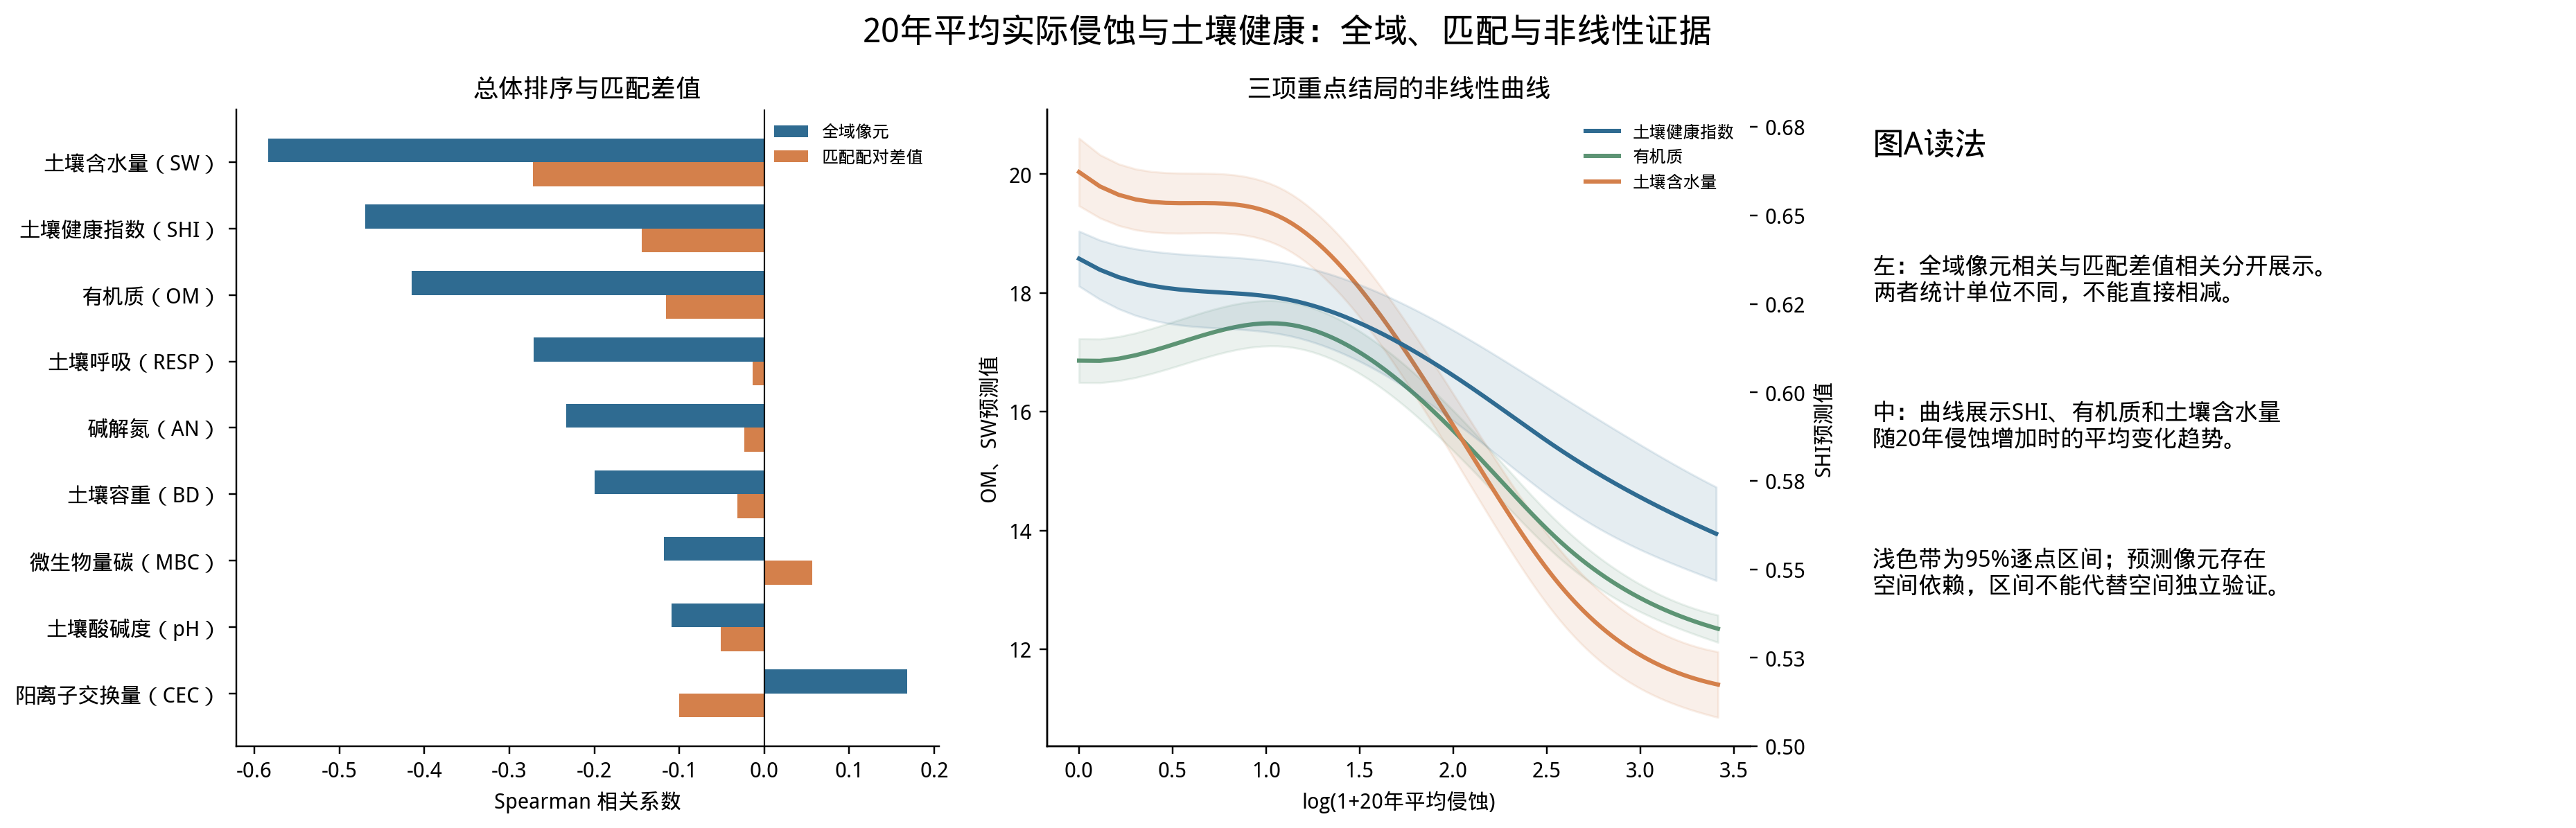
\includegraphics{../figures/A_20yr_global_match_nonlinear.png}
\caption{图A：九项全域相关、匹配差值相关和三项GAM曲线}
\end{figure}

\hypertarget{ux56feb-ux4e5dux9879ux7ed3ux5c40ux7684ux5c40ux90e8ux56deux5f52ux7cfbux6570ux5730ux56fe}{%
\subsubsection{图B
九项结局的局部回归系数地图}\label{ux56feb-ux4e5dux9879ux7ed3ux5c40ux7684ux5c40ux90e8ux56deux5f52ux7cfbux6570ux5730ux56fe}}

\begin{figure}
\centering
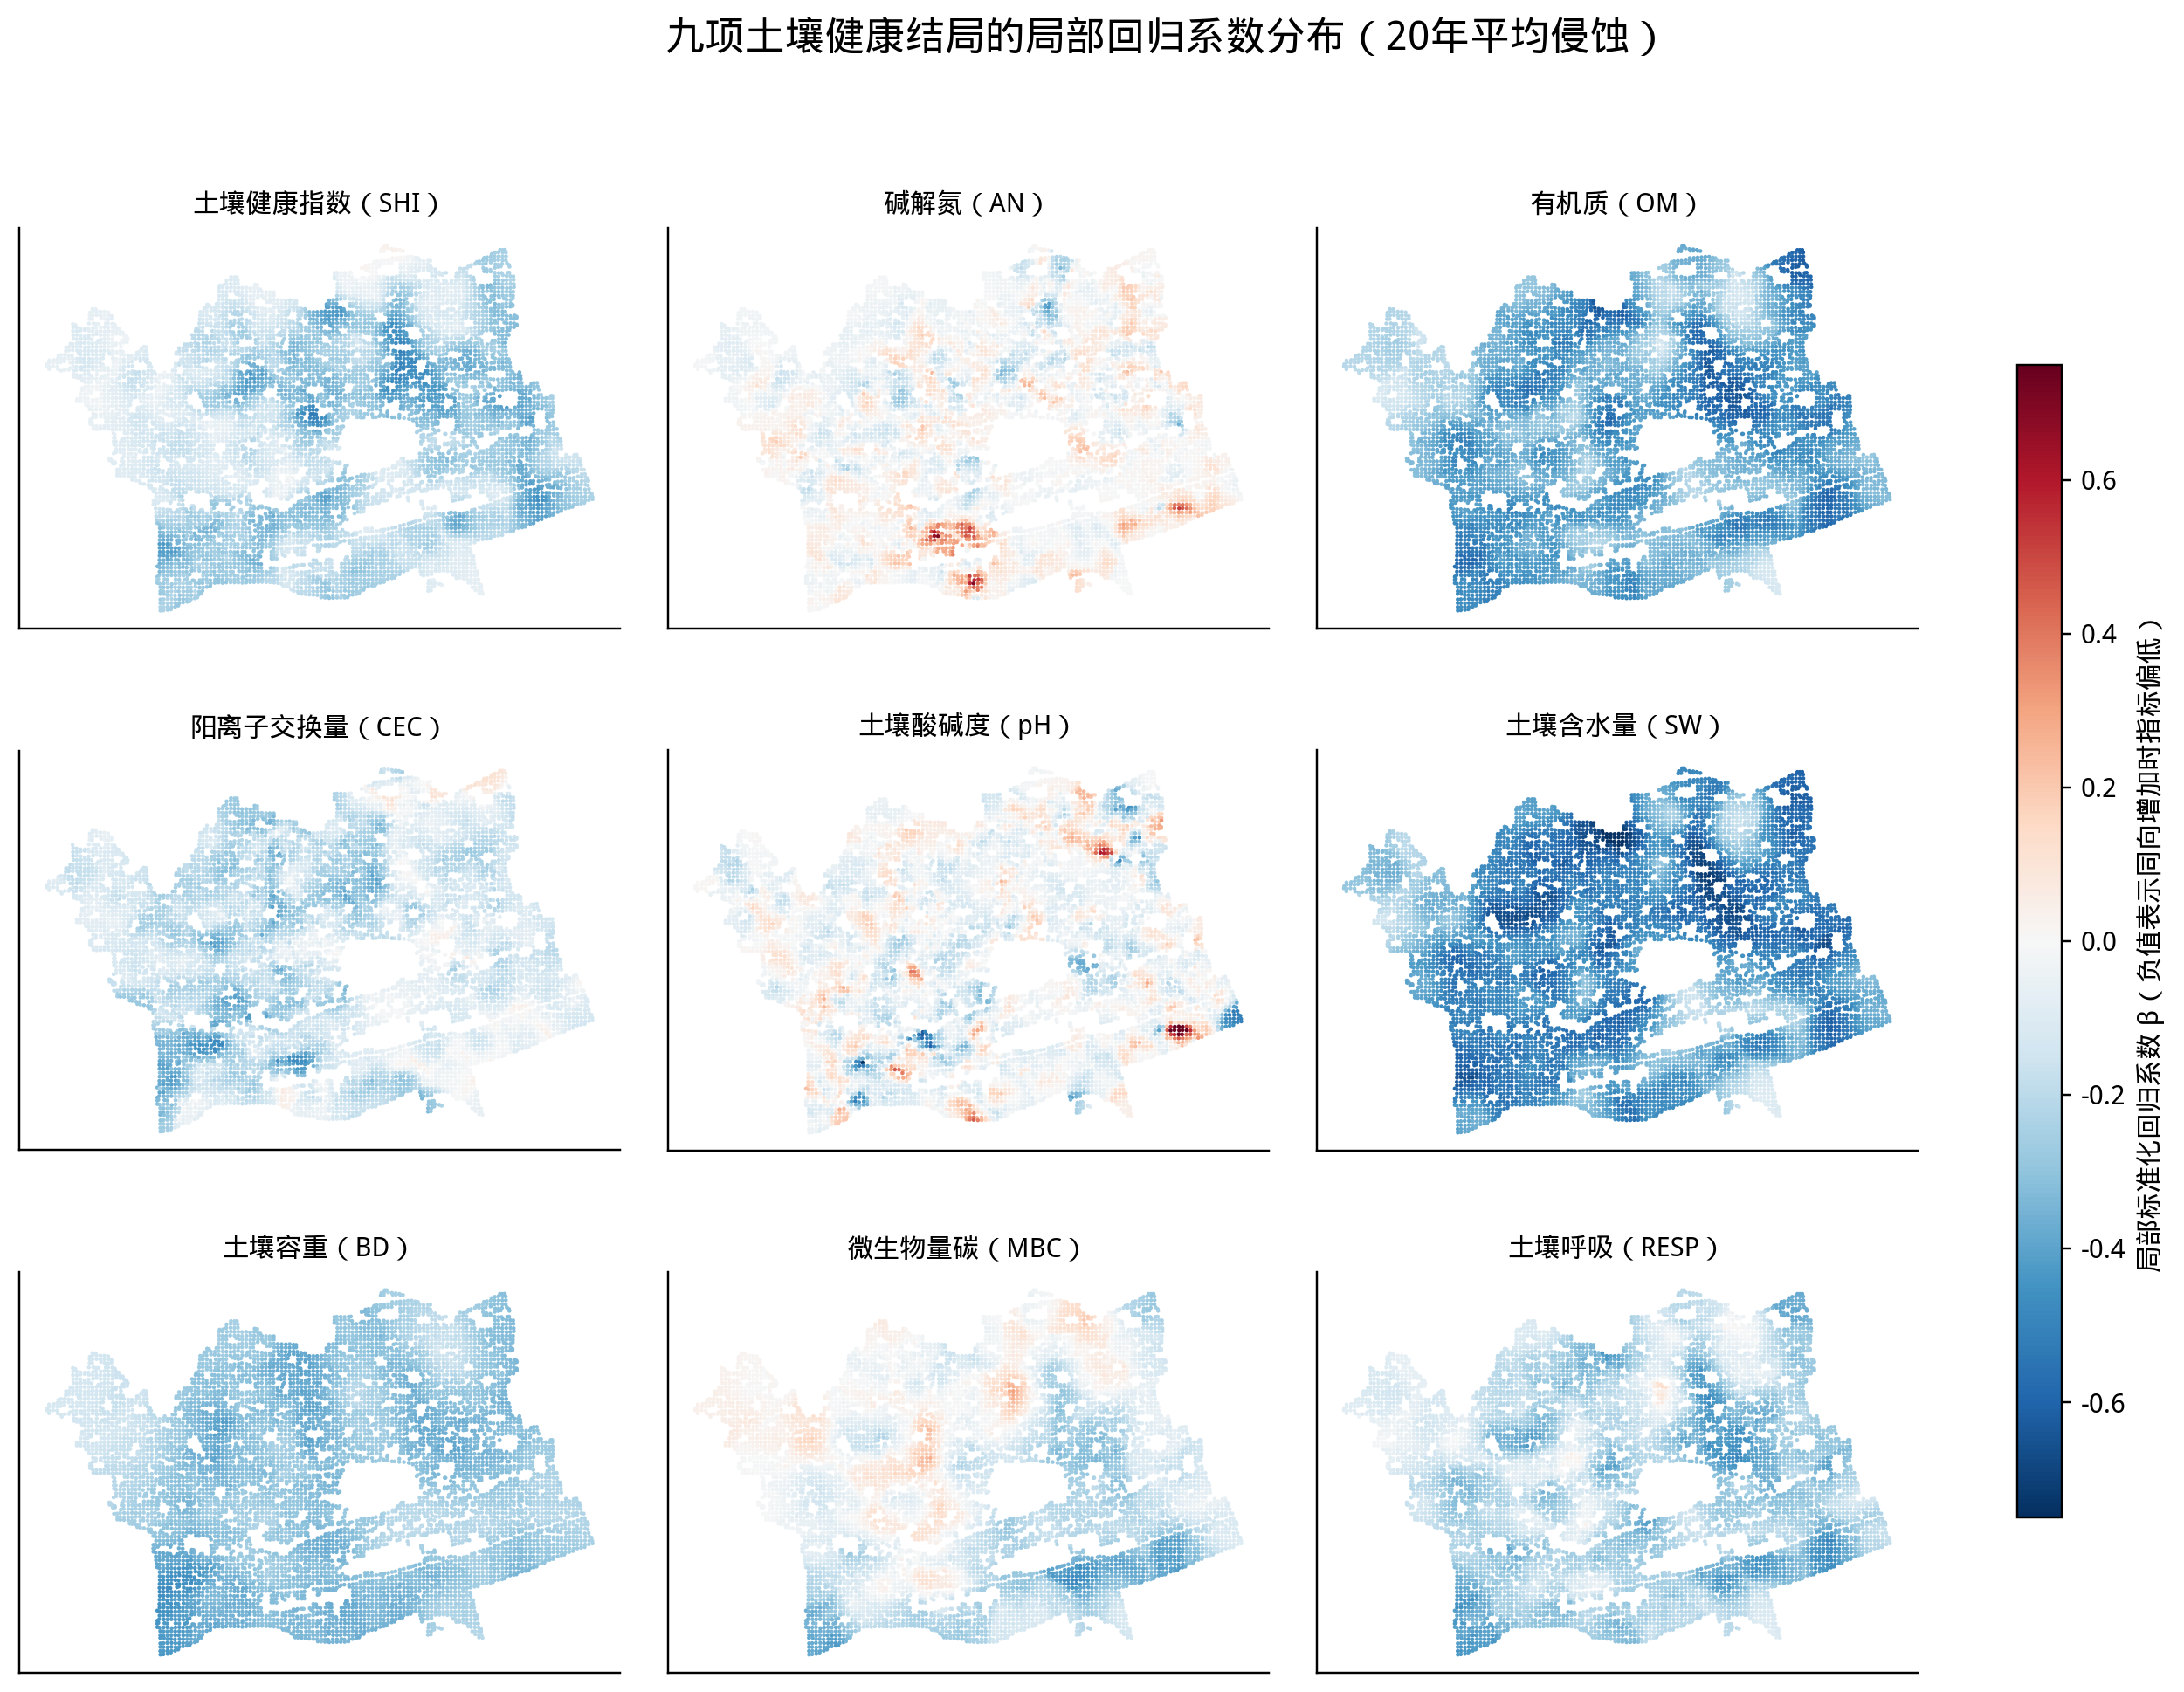
\includegraphics{../figures/B_20yr_nine_outcome_local_maps.png}
\caption{图B：九项结局的局部GWR-LCR系数}
\end{figure}

\hypertarget{ux56fec-ux7a7aux95f4ux654fux611fux4f4dux7f6eux5019ux9009}{%
\subsubsection{图C
空间敏感位置候选}\label{ux56fec-ux7a7aux95f4ux654fux611fux4f4dux7f6eux5019ux9009}}

\begin{figure}
\centering
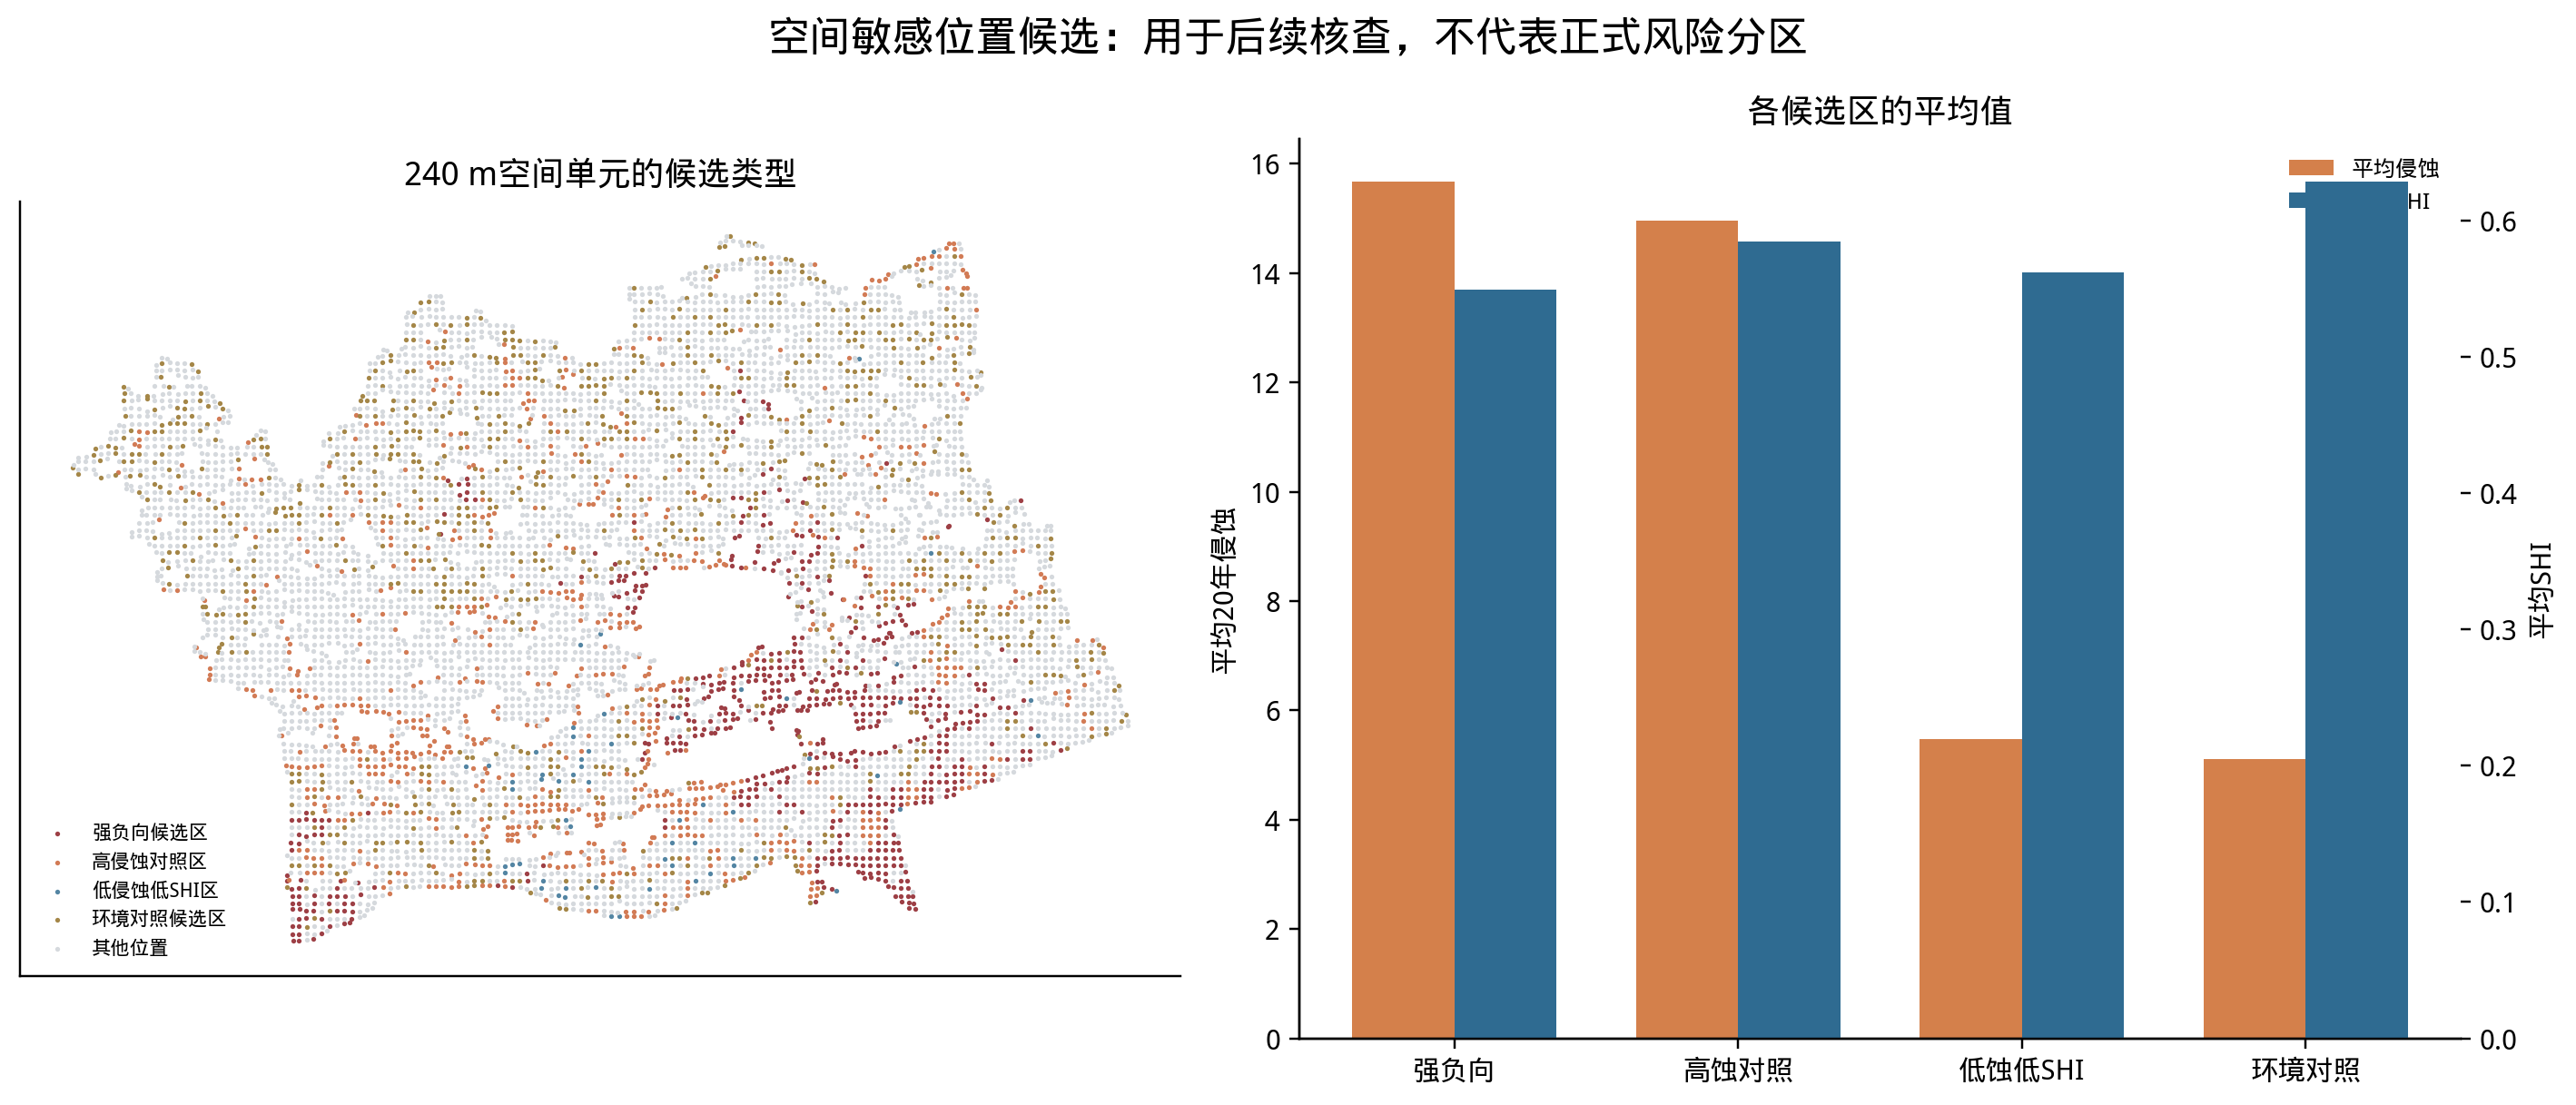
\includegraphics{../figures/C_20yr_candidate_environment_zones.png}
\caption{图C：四类候选区分布及区域均值}
\end{figure}

\hypertarget{ux56fed-ux4e0dux540cux73afux5883ux63a7ux5236ux5c42ux7ea7ux4e0bux7684shiux8defux5f84}{%
\subsubsection{图D
不同环境控制层级下的SHI路径}\label{ux56fed-ux4e0dux540cux73afux5883ux63a7ux5236ux5c42ux7ea7ux4e0bux7684shiux8defux5f84}}

\begin{figure}
\centering
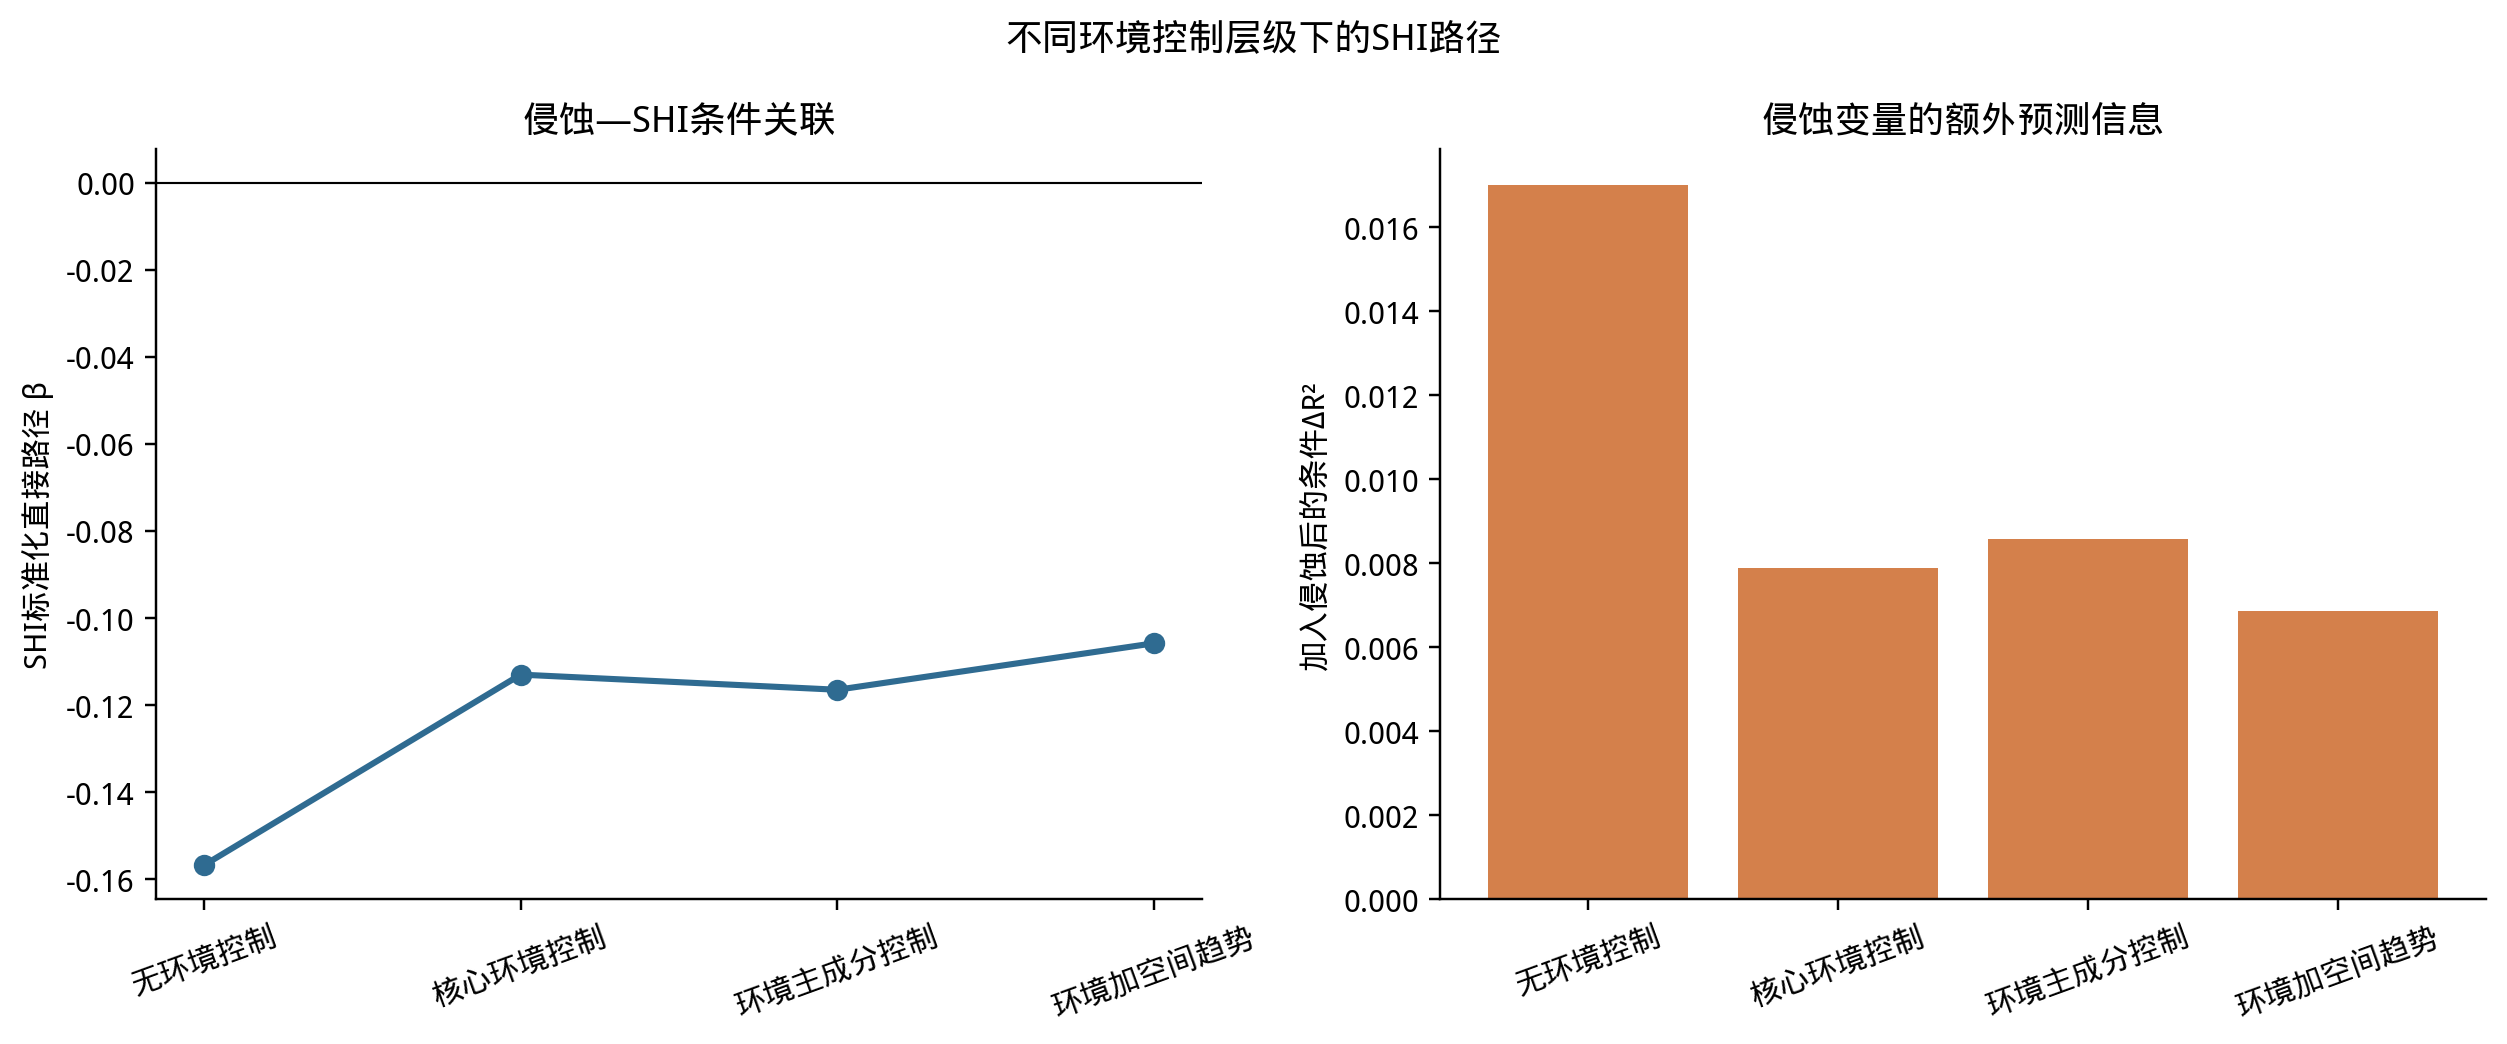
\includegraphics{../figures/D_20yr_sem_control_hierarchy.png}
\caption{图D：不同控制层级下的SHI路径和条件预测增量}
\end{figure}

\hypertarget{ux56fee-ux5168ux57dfux4e0eux5339ux914dux603bux4f53ux7684ux8defux5f84ux5bf9ux7167}{%
\subsubsection{图E
全域与匹配总体的路径对照}\label{ux56fee-ux5168ux57dfux4e0eux5339ux914dux603bux4f53ux7684ux8defux5f84ux5bf9ux7167}}

\begin{figure}
\centering
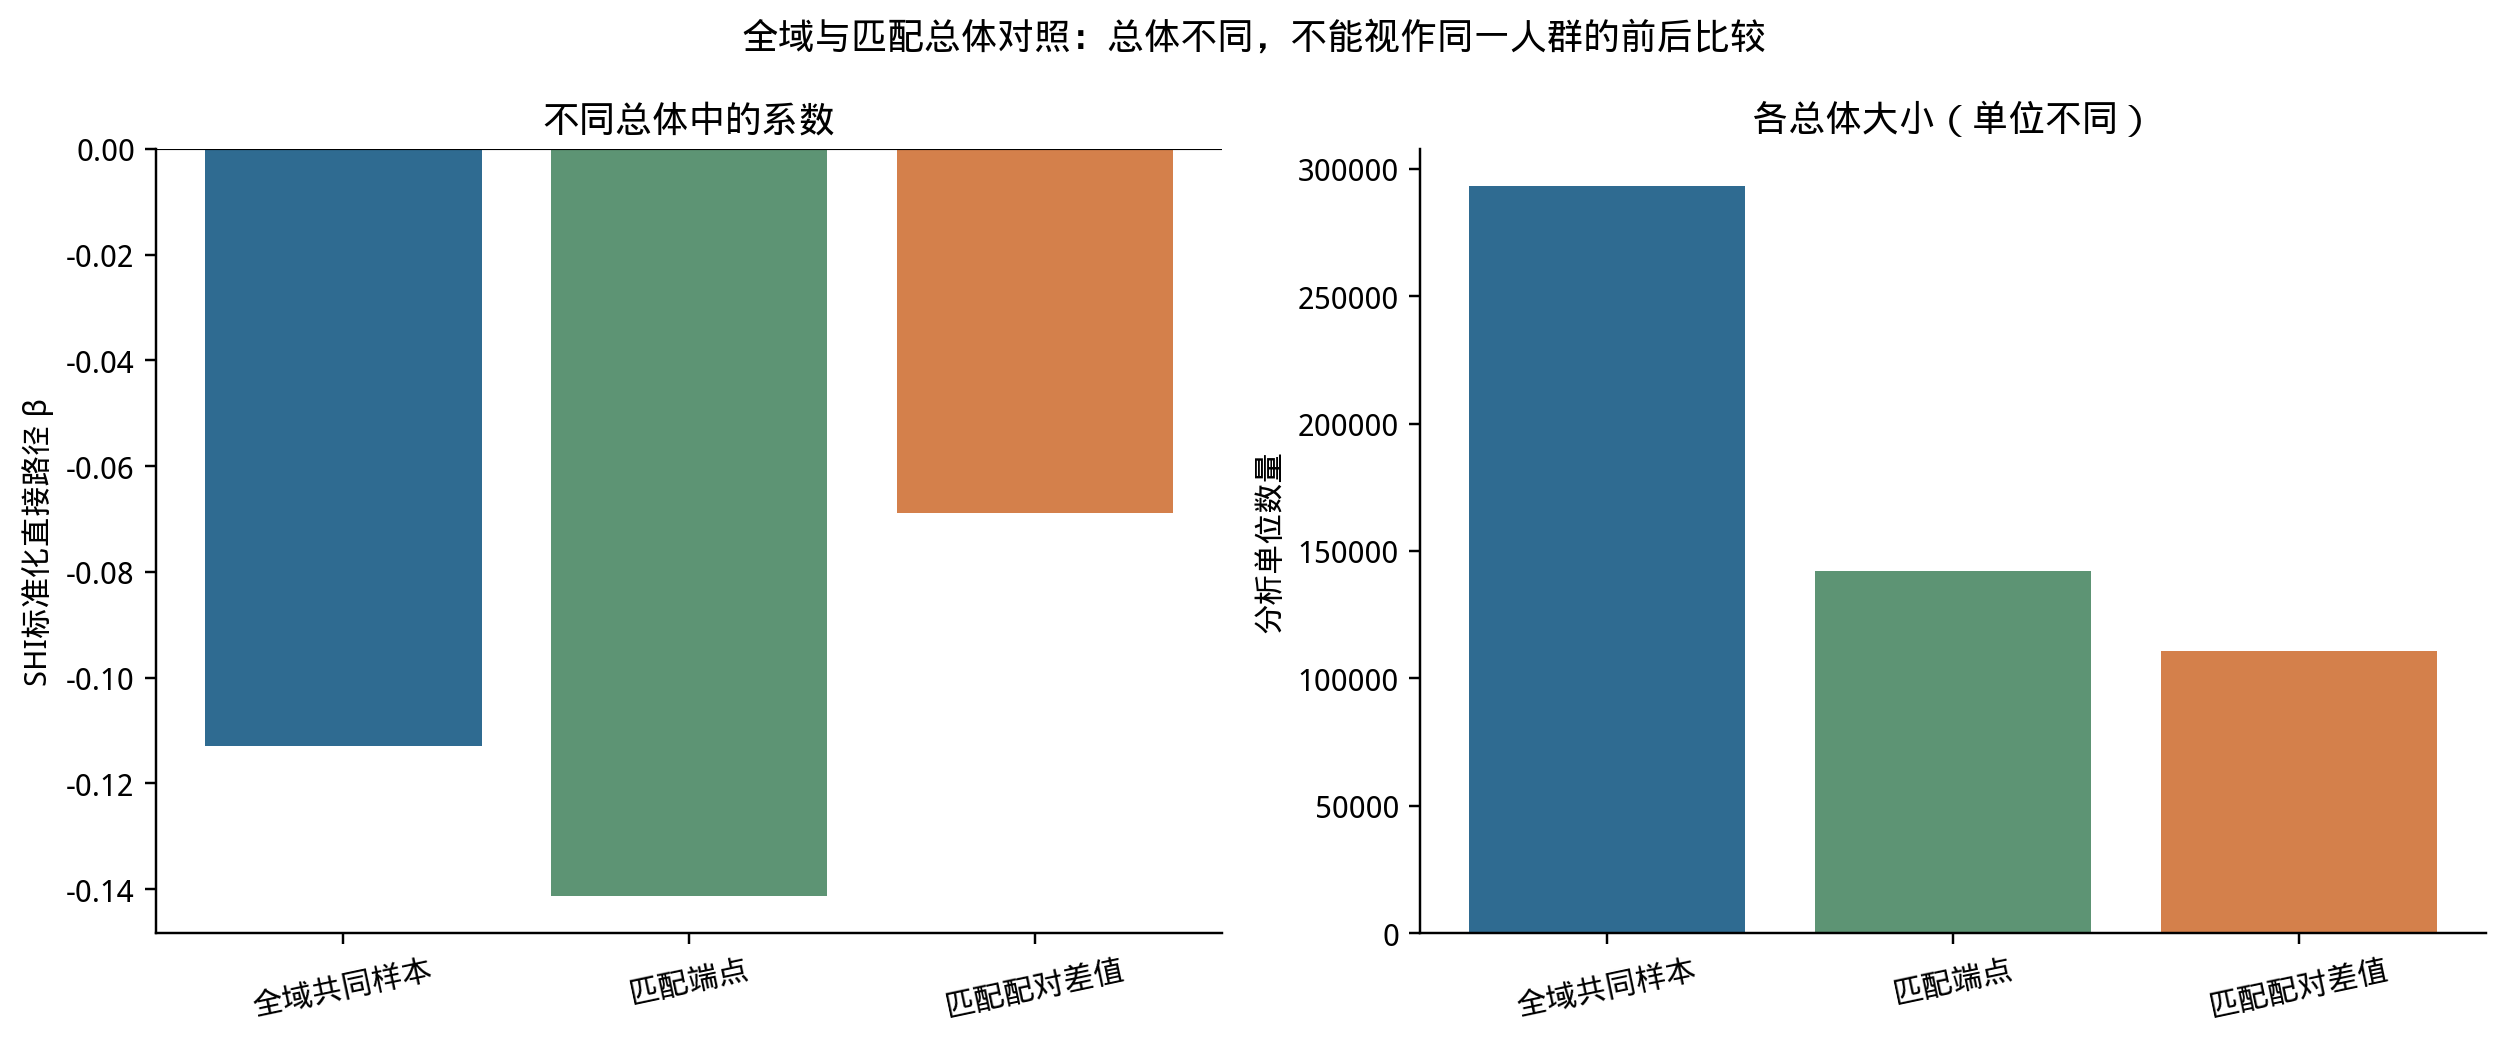
\includegraphics{../figures/E_20yr_full_matched_sem.png}
\caption{图E：全域、匹配端点和匹配差值比较}
\end{figure}

\hypertarget{ux56fef-ux4fb5ux8680ux4e0eux5065ux5eb7ux7ef4ux5ea6ux8defux5f84}{%
\subsubsection{图F
侵蚀与健康维度路径}\label{ux56fef-ux4fb5ux8680ux4e0eux5065ux5eb7ux7ef4ux5ea6ux8defux5f84}}

\begin{figure}
\centering
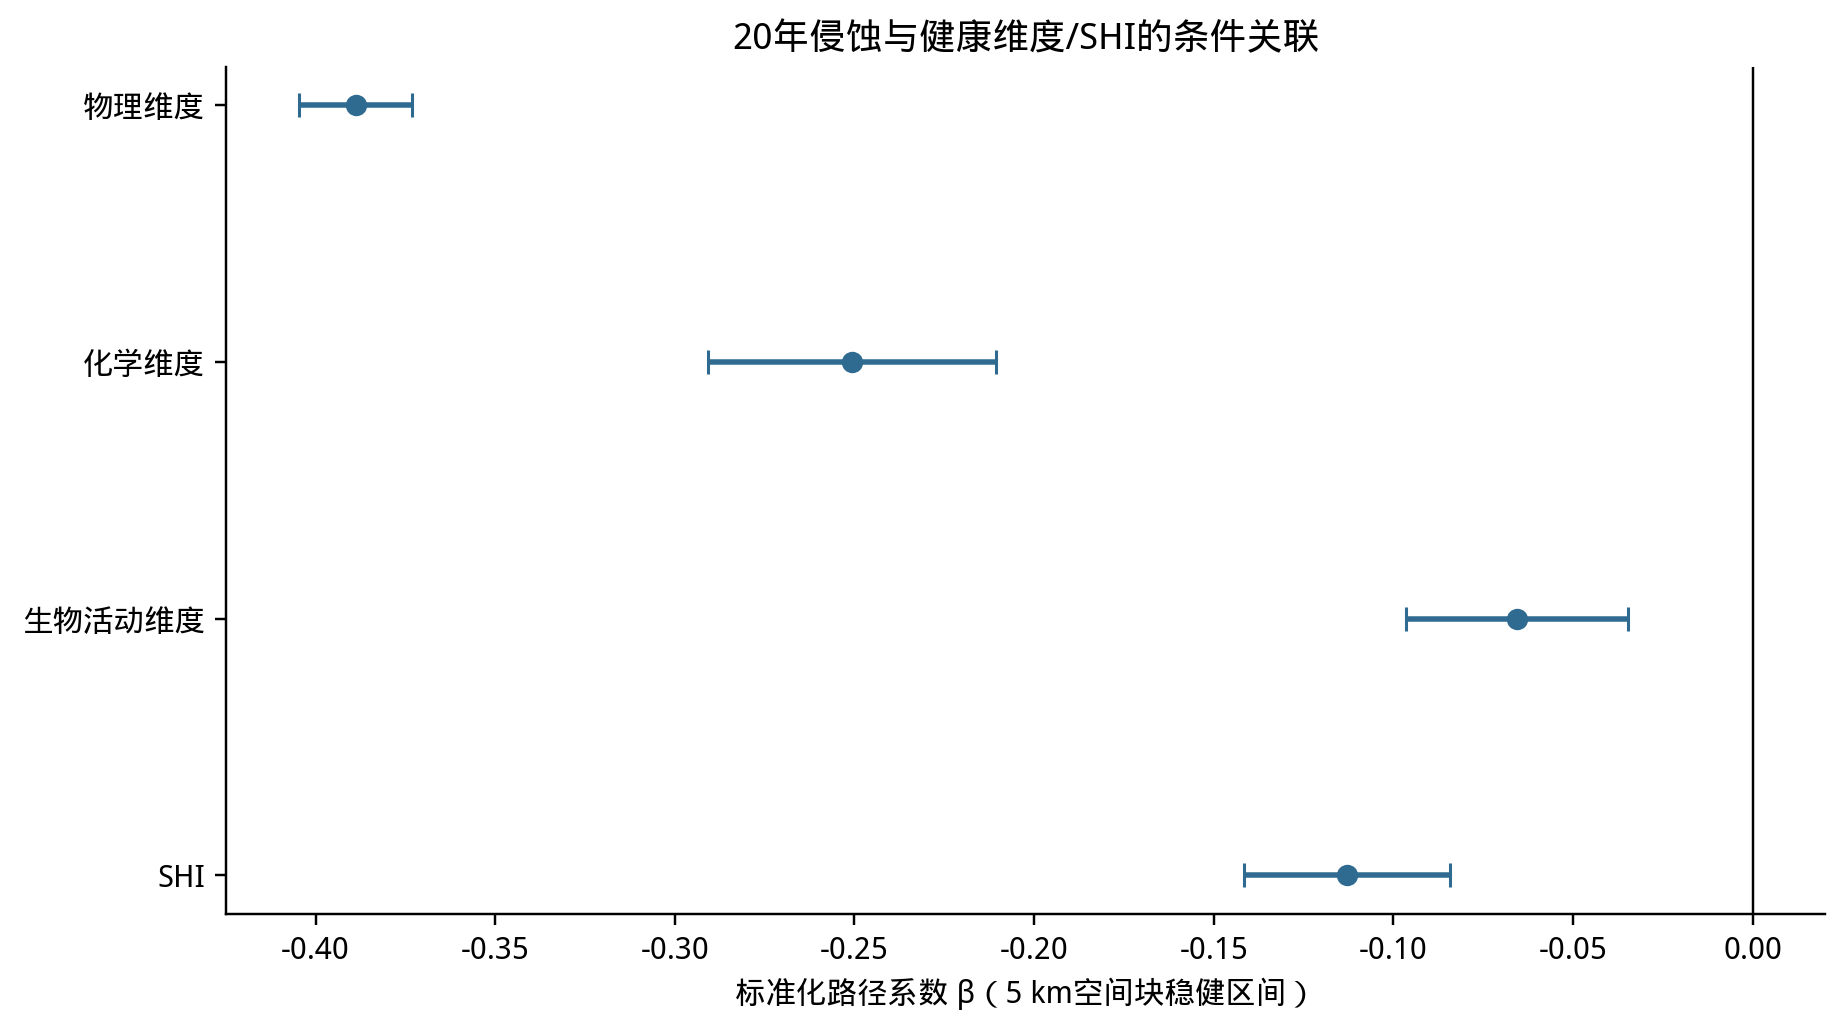
\includegraphics{../figures/F_20yr_sem_dimension_paths.png}
\caption{图F：侵蚀与物理、化学、生物活动及SHI的条件关联}
\end{figure}

\hypertarget{ux56feg-ux73afux5883ux63a7ux5236ux4e0bux7684ux4fb5ux8680ux9884ux6d4bux589eux91cf}{%
\subsubsection{图G
环境控制下的侵蚀预测增量}\label{ux56feg-ux73afux5883ux63a7ux5236ux4e0bux7684ux4fb5ux8680ux9884ux6d4bux589eux91cf}}

\begin{figure}
\centering
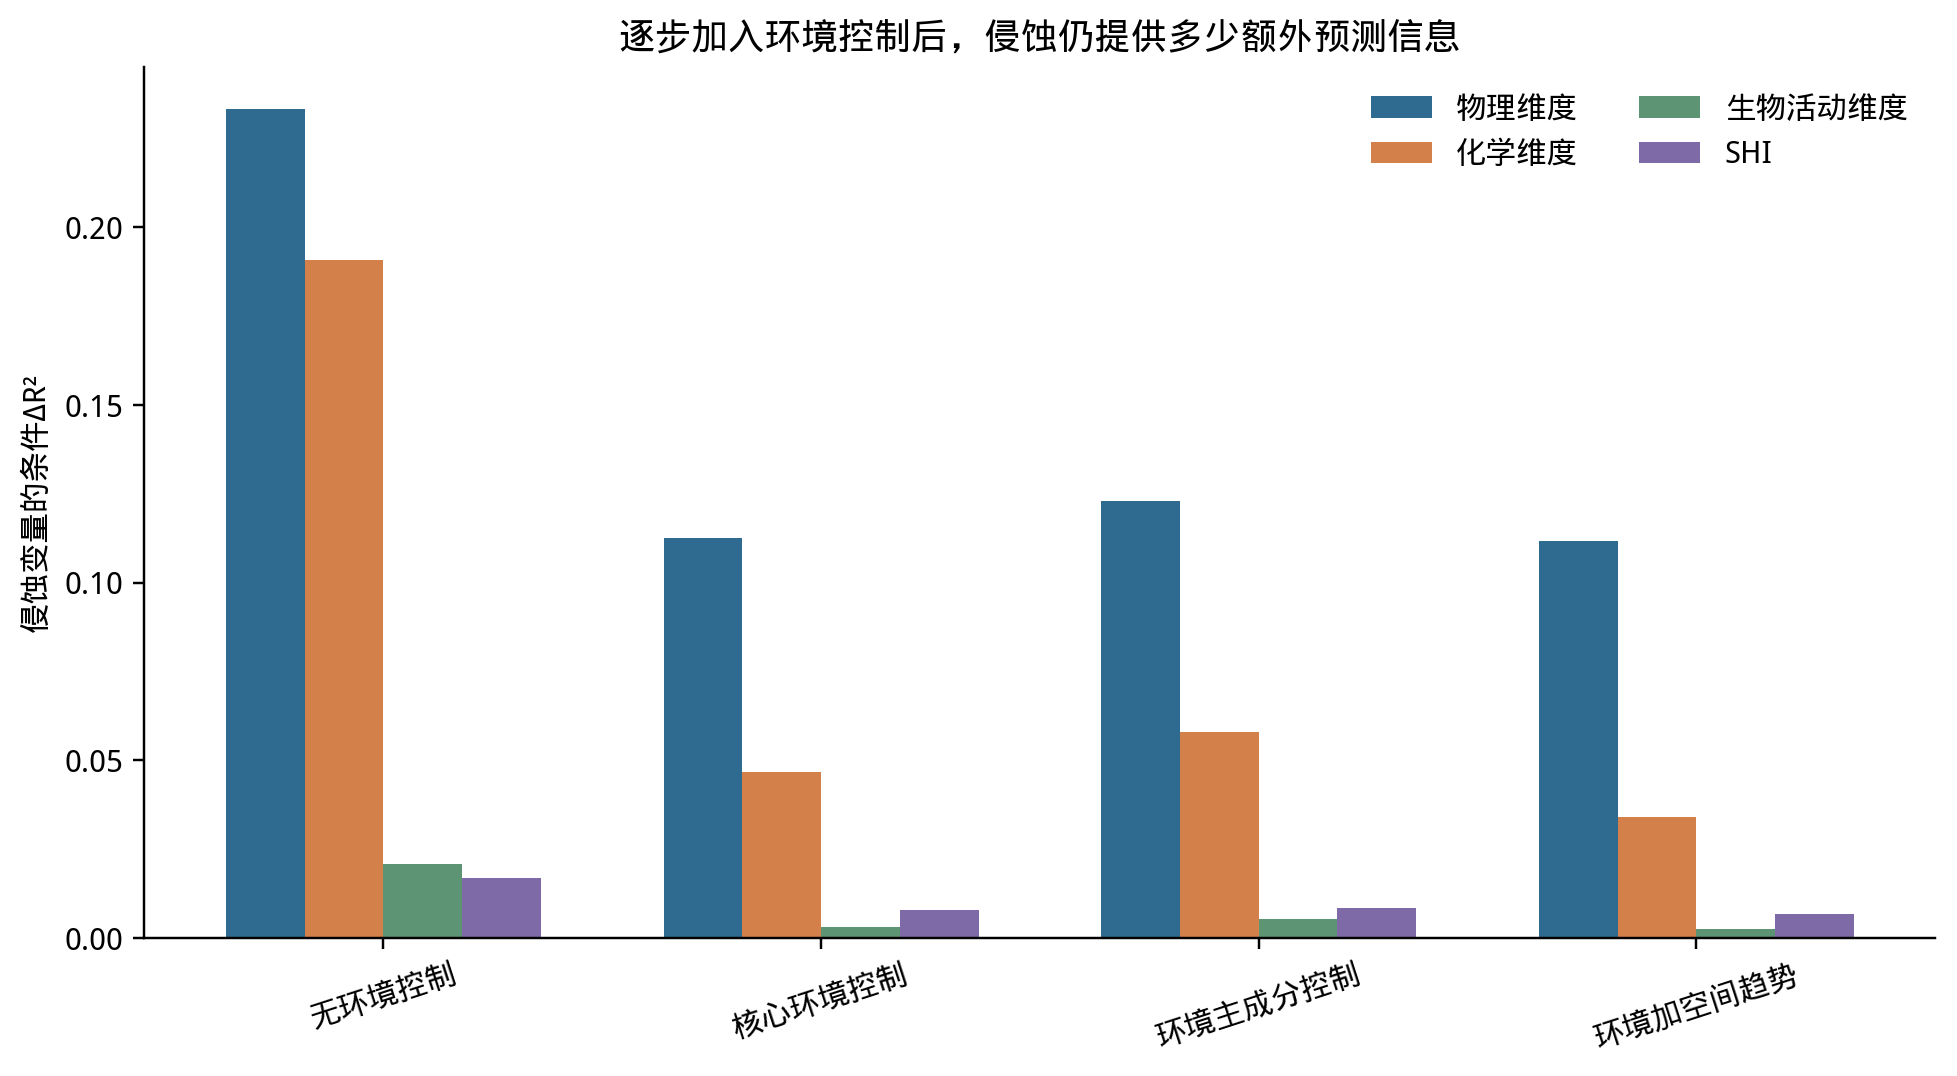
\includegraphics{../figures/G_20yr_sem_incremental_fit.png}
\caption{图G：各控制层级的条件预测增量}
\end{figure}

\hypertarget{ux56feh-ux6838ux5fc3ux7ed3ux6784ux8defux5f84ux56fe}{%
\subsubsection{图H
核心结构路径图}\label{ux56feh-ux6838ux5fc3ux7ed3ux6784ux8defux5f84ux56fe}}

\begin{figure}
\centering
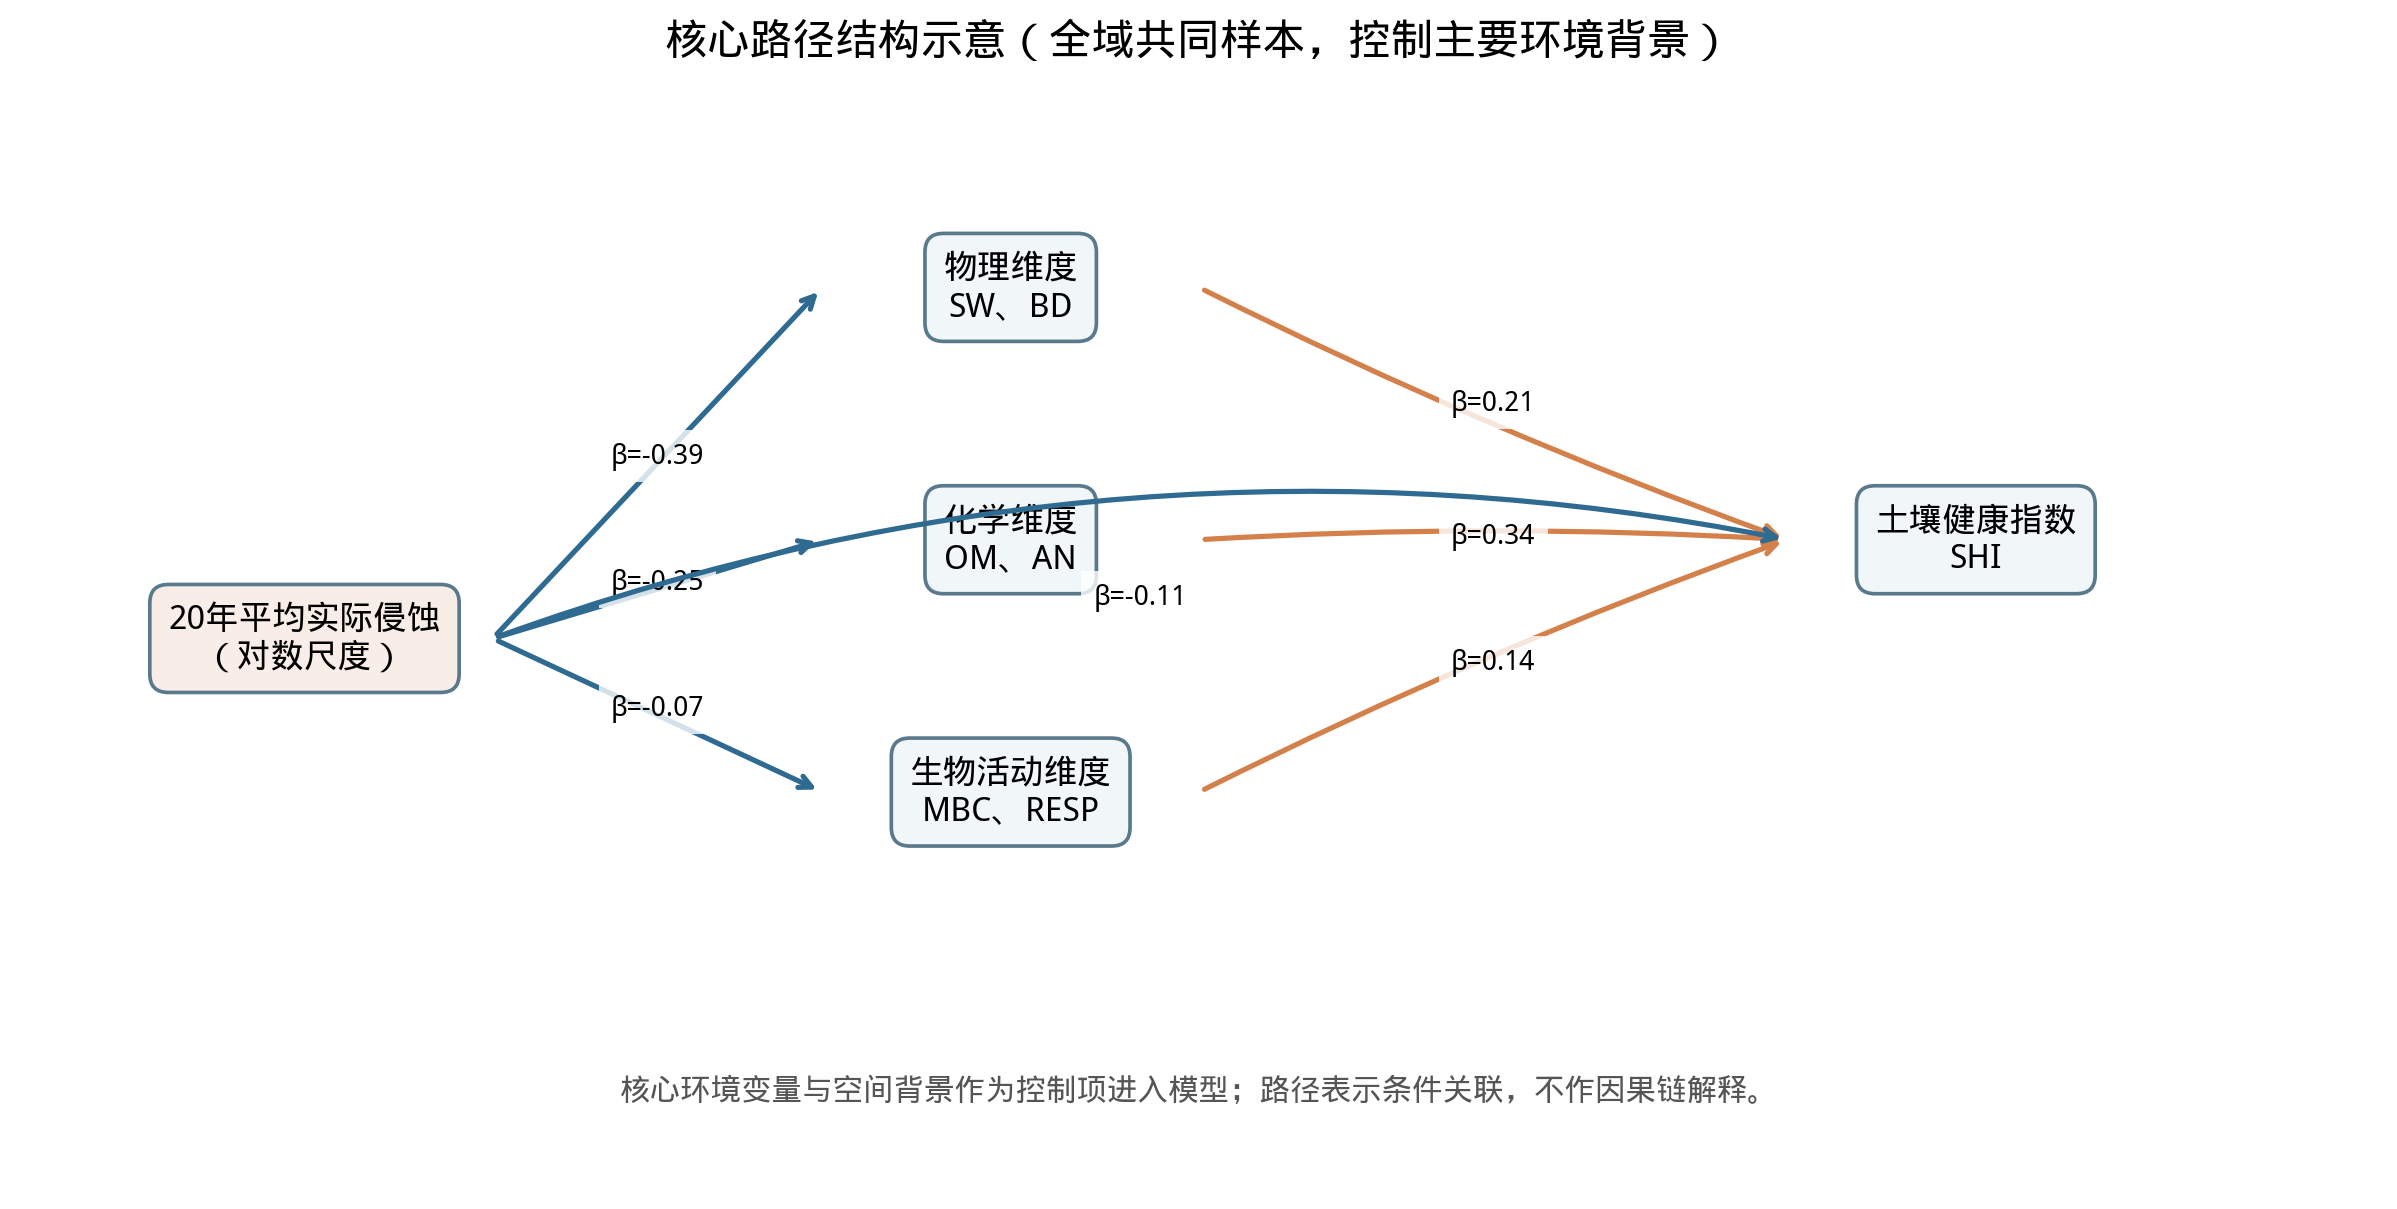
\includegraphics{../figures/H_20yr_sem_path_diagram.png}
\caption{图H：全域共同样本核心路径结构}
\end{figure}

\hypertarget{ux56fei-ux571fux7c7bux4e0eux5730ux5f62ux6e7fux5ea6ux5b50ux7ec4}{%
\subsubsection{图I
土类与地形湿度子组}\label{ux56fei-ux571fux7c7bux4e0eux5730ux5f62ux6e7fux5ea6ux5b50ux7ec4}}

\begin{figure}
\centering
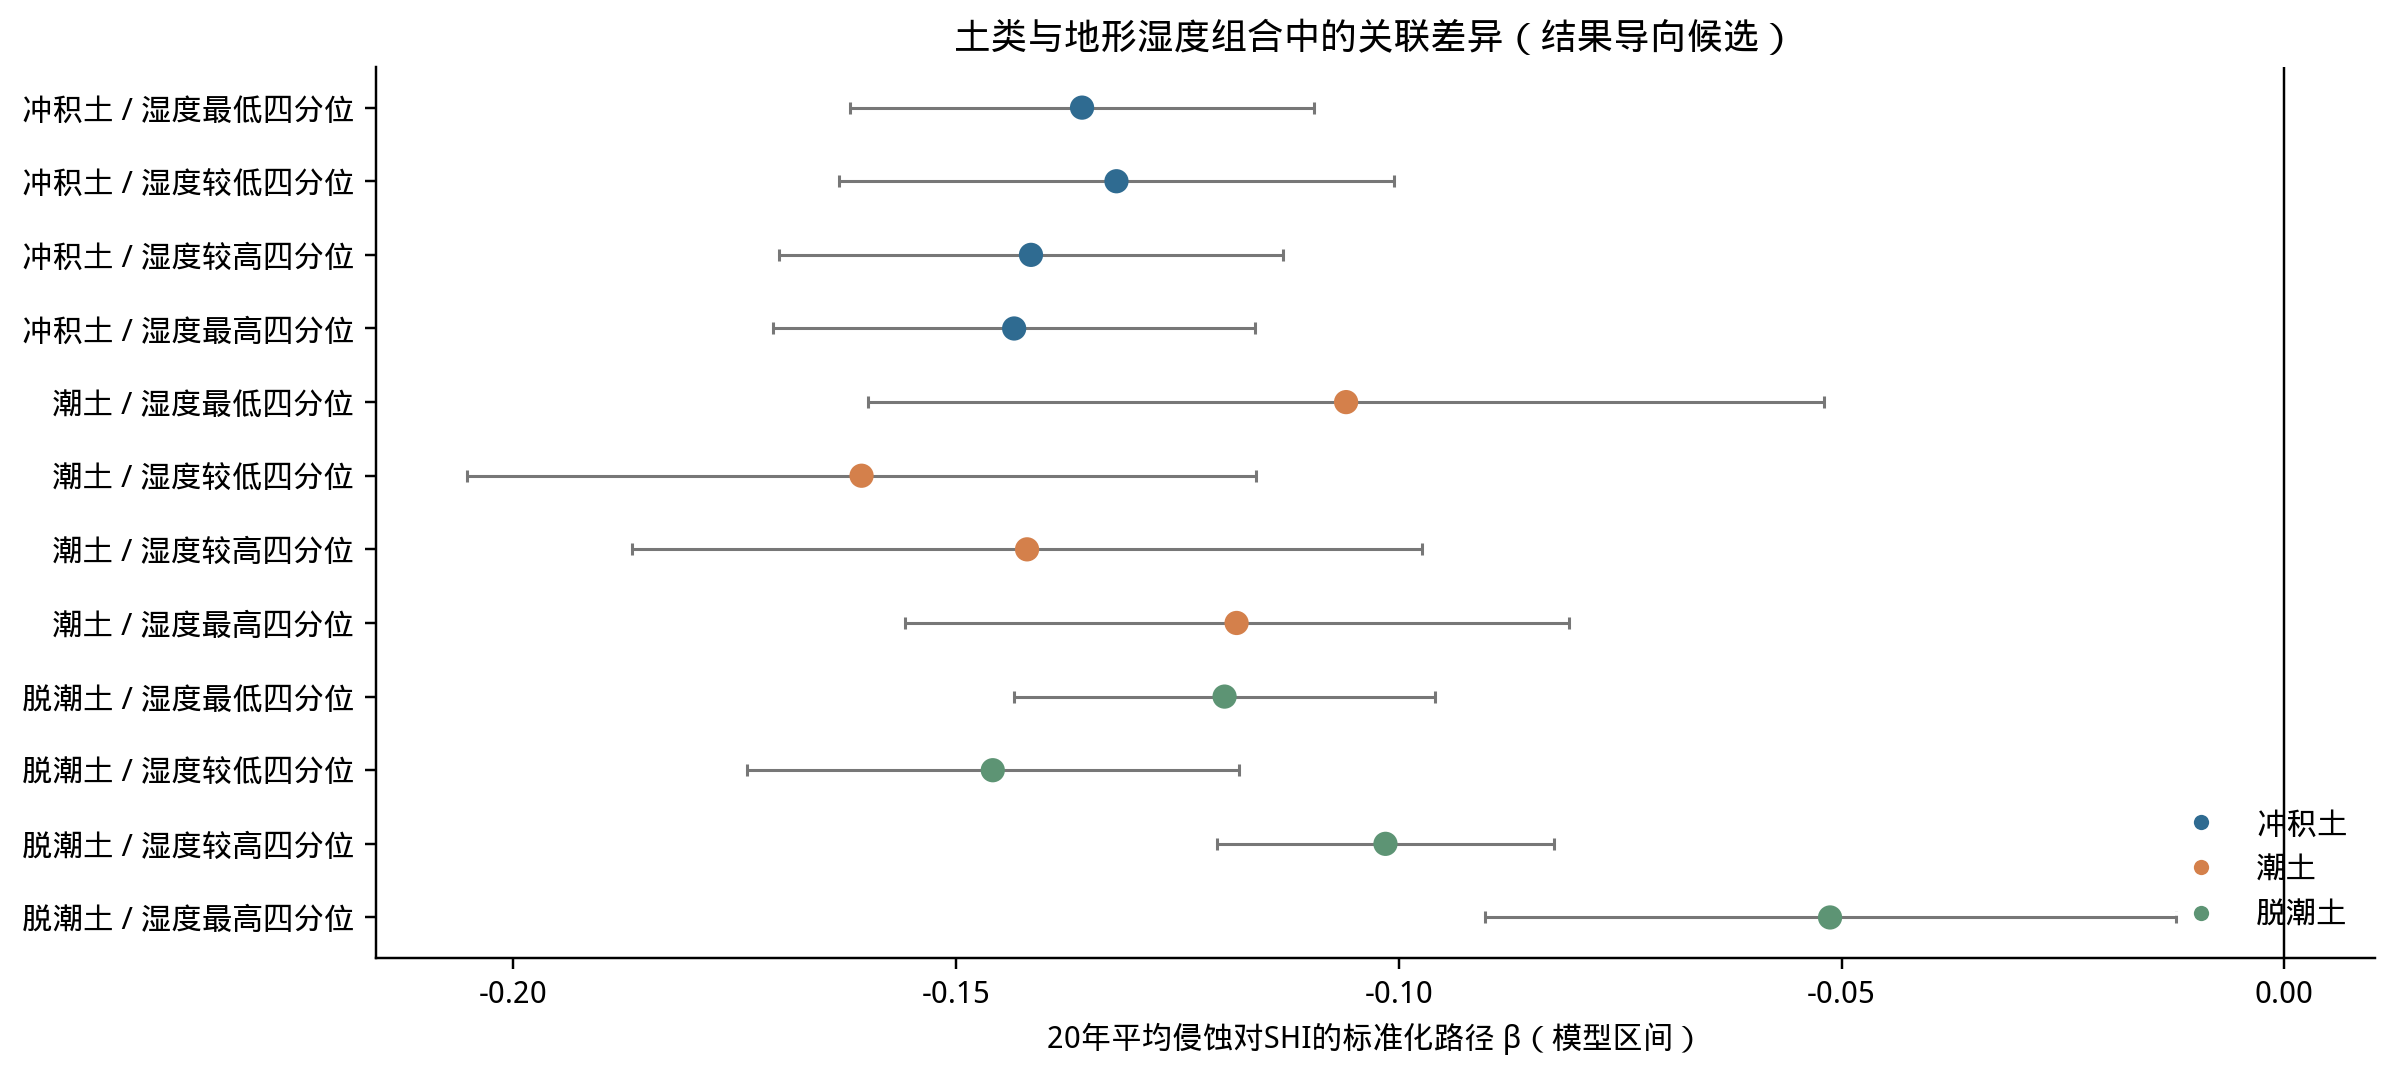
\includegraphics{../figures/I_20yr_soil_twi_sem.png}
\caption{图I：土类和地形湿度组合中的SHI路径}
\end{figure}

\end{document}
